% =====================================================================
% draft.tex — "A New Class of Cellular Automata"
%
% A RESULTS paper, refactored from main.tex (which is an exploration note).
% Joe, 2026-07-17: "I bet we could write a straightforward five-to-ten-page
% paper, including pictures. Rather than 'What Undecidability Feels Like From
% the Inside' I might call it 'A new class of cellular automata'."
%
% WHAT CHANGED, and why. main.tex is 1,197 lines built around a fail bank —
% Joe: "even the fail bank sounds like exploratory data analysis". This keeps
% only what survives as a RESULT and demotes the negatives to the one paragraph
% that explains them.
%
% IN:   the object; the parity theorem; the closed form; fixed-byte counts = 2^k;
%       the census (5x death, monotone in k); the prospective test (reduced
%       rotate+2); bias-not-absorber; the interrupter; and the headline —
%       EVERY FIXED POINT SITS AT LANGTON'S lambda = 1/2, exactly, all 40,320,
%       zero violations, with a two-line proof.
% OUT:  transfer (never shown); the tokamak (cascade 0/12 = identity 0/12, not a
%       win, per lon-claude-6's own control); the duet (MI null); the policy
%       population (blend fired 0.2% of calls); C_mu (a frozen barcode beats
%       Rule 110); the heads (dose 1/80).
% DEMOTED: the three-metric fail bank -> one paragraph. Parity is not a metric
%       property, so distance-geometry cannot see it. That is an explanation,
%       not twenty pages.
% =====================================================================
\documentclass[man,12pt,floatsintext]{apa7}

\usepackage[american]{babel}
\usepackage{csquotes}
\usepackage{amsmath,amssymb}
\usepackage{amsthm}
\usepackage{booktabs}
\usepackage{graphicx}
\usepackage{xcolor}
\usepackage{subcaption}
\usepackage[most]{tcolorbox}
\usetikzlibrary{positioning, arrows.meta, fit}
\usepackage{needspace}
\usepackage[style=apa,backend=biber]{biblatex}
\addbibresource{refs.bib}
\usepackage{nameref}

\newcommand{\sig}{\sigma}
\newcommand{\bit}[1]{\mathrm{bit}[#1]}
% Sections are unnumbered in apa7 `man' mode, so \ref{sec:..} is empty;
% cross-reference sections by name instead.
\newcommand{\secref}[1]{\emph{\nameref{#1}}}
% --- editorial highlighting for review (remove before submission) ---
\newcommand{\discuss}[1]{{\color{blue!65!black}#1}}
\newcommand{\discussnote}[1]{\textcolor{red}{\textbf{[\,DISCUSS: #1\,]}}}
\newtheorem{theorem}{Theorem}
\newtheorem{corollary}{Corollary}
\newtheorem{definition}{Definition}
\newtcolorbox[auto counter]{workedexample}[2][]{%
  enhanced,
  breakable,
  colback=green!6,
  colframe=green!45!black,
  boxrule=0.7pt,
  arc=1.5mm,
  left=2.5mm,
  right=2.5mm,
  top=1.5mm,
  bottom=1.5mm,
  fonttitle=\bfseries,
  title={Worked example~\thetcbcounter: #2},
  #1}

% --- typed boxes for compression -------------------------------------------
% Auto-box existing amsthm theorems/definitions (no source change; keeps refs).
\tcolorboxenvironment{theorem}{%
  enhanced, breakable, colback=blue!5, colframe=blue!55!black,
  boxrule=0.7pt, arc=1.5mm, left=2.5mm, right=2.5mm, top=1.5mm, bottom=1.5mm}
\tcolorboxenvironment{definition}{%
  enhanced, breakable, colback=violet!6, colframe=violet!55!black,
  boxrule=0.7pt, arc=1.5mm, left=2.5mm, right=2.5mm, top=1.5mm, bottom=1.5mm}
% Exposition box (blue): non-claim prose that aids comprehension. Its title is a
% headline stating what the passage adds. Break a long one into \pointbox points.
\newtcolorbox{expositionbox}[2][]{%
  enhanced, breakable, colback=blue!3, colframe=blue!45!black,
  boxrule=0.5pt, arc=1.2mm, left=2.5mm, right=2.5mm, top=1.5mm, bottom=1.5mm,
  fonttitle=\bfseries, coltitle=white, title={#2}, #1}
\newtcolorbox{pointbox}[1]{%
  enhanced, colback=white, colframe=gray!45,
  boxrule=0.4pt, arc=0.8mm, left=2mm, right=2mm, top=0.8mm, bottom=0.8mm,
  fonttitle=\bfseries\small, coltitle=black, title={#1}}
% Corollaries auto-boxed like theorems (blue). Empirical findings are amber:
% observed (not proved) claims live here, the validated home for rewritten results.
\tcolorboxenvironment{corollary}{%
  enhanced, breakable, colback=blue!5, colframe=blue!55!black,
  boxrule=0.7pt, arc=1.5mm, left=2.5mm, right=2.5mm, top=1.5mm, bottom=1.5mm}
\newtcolorbox[auto counter]{empiricalfinding}[2][]{%
  enhanced, breakable, colback=orange!7, colframe=orange!65!black,
  boxrule=0.7pt, arc=1.5mm, left=2.5mm, right=2.5mm, top=1.5mm, bottom=1.5mm,
  fonttitle=\bfseries, title={Empirical finding~\thetcbcounter: #2}, #1}
% Observations (teal): consequences/remarks pulled out of definitions and prose.
\newtcolorbox[auto counter]{observation}[2][]{%
  enhanced, breakable, colback=teal!7, colframe=teal!55!black,
  boxrule=0.7pt, arc=1.5mm, left=2.5mm, right=2.5mm, top=1.5mm, bottom=1.5mm,
  fonttitle=\bfseries, title={Observation~\thetcbcounter: #2}, #1}

\title{A New Family of Operators on Cellular Automata}
\shorttitle{A New Family of Operators on Cellular Automata}
\author{Joseph Corneli}
\affiliation{}

\abstract{%
We describe a cellular automaton whose cells hold not states but \emph{rules},
and an operator $P_\sig$ that rewrites each rule by acting on its own truth table,
$\bit{\sig(k)} := \lnot\,\bit{k}$ for $\sig$ a permutation of the eight
neighbourhoods (Def.~\ref{def:writing}). This gives a finite, exhaustively
classifiable family of $8! = 40{,}320$ operators---a vanishing $0.24\%$ of the
general \emph{writings} (Obs.~\ref{obs:core}).

The classification is exact and machine-checked: $P_\sig$ has a fixed rule if and
only if every cycle of $\sig$ is even (Thm.~\ref{thm:parity}), and every fixed
rule is \emph{balanced}, at Langton's $\lambda = 1/2$ (Thm.~\ref{thm:lambda}). A
census of all $40{,}320$ makes this a measured law: any odd cycle forbids
collapse, the all-even class splits, and every genotype/phenotype regime is
reachable by a bijection (Table~\ref{tab:census}).

Balance is exact, but edge-of-chaos \emph{behaviour} is a separate question: only
the coprime 8-cycles sustain a high-diversity phase (Emp.~find.~\ref{find:survey},
Fig.~\ref{fig:eoc}). That phase has no critical point but a finite-width
\emph{littoral edge} (Emp.~find.~\ref{find:crossover},~\ref{find:littoral};
Fig.~\ref{fig:phase}), whose
ordered and chaotic domains meet at fractal walls where the genotype is rewritten
fastest (Emp.~find.~\ref{find:walls}, Fig.~\ref{fig:interface}). The family is
flat under its own composition (Obs.~\ref{obs:flat}); yet pairing a propagator
with a construction step---a \emph{river}---or braiding complementary operators
nonetheless manufactures sustained structure (Figs.~\ref{fig:braid},
\ref{fig:river}).}

\begin{document}
\maketitle

\section{The Object}
\label{sec:object}

A cellular automaton normally evolves a field of \emph{states} under one
fixed rule. Invert that arrangement: let each cell hold a \emph{rule}, and
let an operator evolve the field of rules. An elementary cellular automaton
(ECA) rule is an eight-bit truth table $\bit{k}$, with $k$ ranging over the
eight three-cell neighbourhoods. We study the operator $P_\sig$, parameterised by a
permutation $\sig \in S_8$ that acts on the rule's own table. Writing a rule
as a map $g\colon \{0,\dots,7\} \to \{0,1\}$, the operator sends $g$ to
$P_\sig g$ defined by
\begin{equation}
(P_\sig\, g)(j) \;=\; \lnot\, g\bigl(\sig^{-1}(j)\bigr),
\qquad\text{equivalently}\qquad \bit{\sig(k)} := \lnot\,\bit{k}.
\label{eq:prop}
\end{equation}
Each output bit is one input bit, at the position $\sig$ moves it to, negated;
$P_\sig$ is thus a permutation of the eight coordinates composed with a global
complement. The truth table is thereby itself an eight-cell automaton whose
wiring is $\sig$ and whose update is Boolean negation --- an automaton inside
the automaton. Equation~\eqref{eq:prop} defines a family of $8! = 40{,}320$
operators that is finite, exhaustively enumerable, and, as we show below,
exactly classified.

\begin{definition}[Writings, propagators, and permutations]\label{def:writing}
A \emph{writing} is any function $w\colon\{0,\dots,7\}\to\{0,\dots,7\}$ on the
truth-table positions, and its \emph{propagator} $P_w$ complements each source
bit and writes it to the target $w(k)$: $\bit{w(k)} := \lnot\,\bit{k}$. When $w$
is a bijection---a permutation $\sig\in S_8$---each target is written exactly
once, $\sig^{-1}$ exists, and $P_\sig$ takes the closed form~\eqref{eq:prop};
these are the \emph{permutation-propagators}. A non-injective writing has
\emph{collisions} (two sources sharing a target, so the simultaneous rewrite is
order-dependent) and \emph{gaps} (a position written by none).
\end{definition}

\begin{observation}[label={obs:core}]{The permutation core is a vanishing fraction}
Permutations are only the bijective core of a far larger class: there are
$8!=40{,}320$ permutations but $8^{8}=16{,}777{,}216$ writings, so the
permutations are $0.24\%$ of the whole. The cycle-structure algebra of
\secref{sec:classification} is available only on this core. The historical
operator $[0\,0\,1\,2\,3\,4\,5\,6]$ (Figure~\ref{fig:fig2pair}) is itself a
non-bijective writing---bits $0$ and $1$ both write to position $0$, and
position $7$ is never written---and its behaviour ranges widely between its two
standard-order forms.
\end{observation}

\begin{figure}[!tp]
\centering
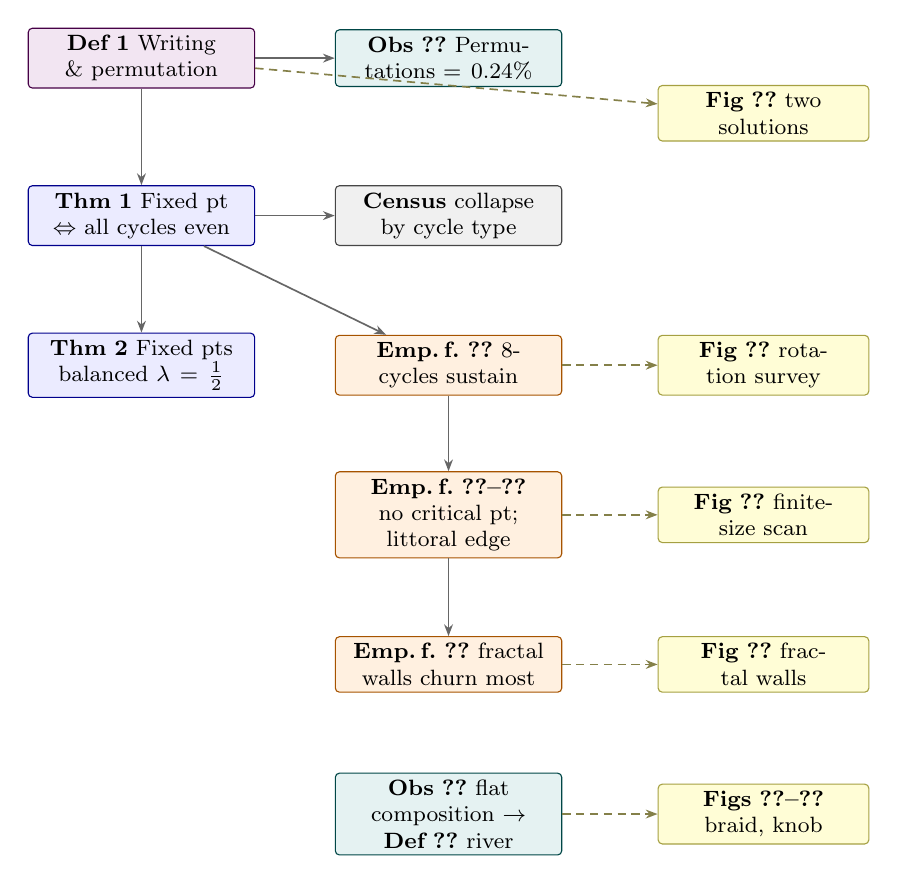
\begin{tikzpicture}[font=\footnotesize, >={Stealth[length=1.5mm]},
  bx/.style={draw, rounded corners=1.5pt, align=center, inner sep=2.5pt,
             text width=27mm, minimum height=7mm},
  defn/.style={bx, fill=violet!10, draw=violet!55!black},
  thm/.style={bx, fill=blue!8, draw=blue!55!black},
  obs/.style={bx, fill=teal!10, draw=teal!55!black},
  ef/.style={bx, fill=orange!12, draw=orange!65!black},
  cen/.style={bx, fill=gray!12, draw=gray!55!black},
  fig/.style={bx, fill=yellow!16, draw=yellow!60!black, text width=25mm},
  s/.style={->, draw=black!60, semithick},
  v/.style={->, draw=yellow!45!black, semithick, densely dashed}]
% proved core (left)
\node[defn] (d1) at (0,0)    {\textbf{Def 1} Writing \& permutation};
\node[thm]  (t1) at (0,-2.0) {\textbf{Thm 1} Fixed pt $\Leftrightarrow$ all cycles even};
\node[thm]  (t2) at (0,-3.9) {\textbf{Thm 2} Fixed pts balanced $\lambda=\tfrac12$};
% object + measured + constructive (center)
\node[obs] (obs1) at (3.9,0)    {\textbf{Obs~\ref{obs:core}} Permutations $=0.24\%$};
\node[cen] (cen)  at (3.9,-2.0) {\textbf{Census} collapse by cycle type};
\node[ef]  (efs)  at (3.9,-3.9) {\textbf{Emp.\,f.~\ref{find:survey}} 8-cycles sustain};
\node[ef]  (efl)  at (3.9,-5.8) {\textbf{Emp.\,f.~\ref{find:crossover}--\ref{find:littoral}} no critical pt; littoral edge};
\node[ef]  (efw)  at (3.9,-7.7) {\textbf{Emp.\,f.~\ref{find:walls}} fractal walls churn most};
\node[obs] (obsf) at (3.9,-9.6) {\textbf{Obs~\ref{obs:flat}} flat composition $\to$ \textbf{Def~\ref{def:river}} river};
% figures (right): what each claim rests on
\node[fig] (ff2) at (7.9,-0.7) {\textbf{Fig~\ref{fig:fig2pair}} two solutions};
\node[fig] (feoc)at (7.9,-3.9) {\textbf{Fig~\ref{fig:eoc}} rotation survey};
\node[fig] (fph) at (7.9,-5.8) {\textbf{Fig~\ref{fig:phase}} finite-size scan};
\node[fig] (fint)at (7.9,-7.7) {\textbf{Fig~\ref{fig:interface}} fractal walls};
\node[fig] (fbr) at (7.9,-9.6) {\textbf{Figs~\ref{fig:braid}--\ref{fig:knob}} braid, knob};
% support (solid) + visual-evidence (dashed) edges
\draw[s] (d1)--(t1); \draw[s] (t1)--(t2); \draw[s] (d1)--(obs1);
\draw[s] (t1)--(cen); \draw[s] (t1)--(efs);
\draw[s] (efs)--(efl); \draw[s] (efl)--(efw);
\draw[v] (d1)--(ff2); \draw[v] (efs)--(feoc); \draw[v] (efl)--(fph);
\draw[v] (efw)--(fint); \draw[v] (obsf)--(fbr);
\end{tikzpicture}
\caption{\textbf{Map of the paper by box.} Solid arrows carry logical support;
\emph{dashed} arrows link each claim to the \textbf{figure} that visualises it
(yellow)---the argument rests on what can be seen. Colour encodes type:
definition (violet), theorem (blue), observation (teal), empirical finding
(amber), census (grey), figure (yellow). Only the principal boxes are drawn; the
paper carries some two dozen typed boxes in all, plus exposition boxes for the
connecting prose. Anything not in a box is droppable scaffolding.}
\label{fig:map}
\end{figure}

Box~\ref{box:propagator} works through one member of the
family bit by bit.

\begin{workedexample}[label={box:propagator}]{A propagator by hand}
\small
Write an ECA rule in Wolfram's standard neighbourhood order:
\begin{center}
\setlength{\tabcolsep}{3.2pt}
\begin{tabular}{c@{\quad}*{8}{c}}
neighbourhood & $111$ & $110$ & $101$ & $100$ & $011$ & $010$ & $001$ & $000$ \\
\midrule
Rule 110 & $0$ & $1$ & $1$ & $0$ & $1$ & $1$ & $1$ & $0$ \\
\end{tabular}
\end{center}
Thus Rule~110 is the byte $01101110$. Let $\sig(k)=k+2\pmod 8$:
each source bit is complemented and written two positions further along.
Carrying out the eight writes gives
\[
P_{+2}(01101110)=01100100,
\]
which is Rule~100. This changes what the cell does to its black-and-white
phenotype. For example, neighbourhood $011$ maps to $1$ under Rule~110 but
to $0$ under Rule~100. The propagator has not directly flipped a phenotype
cell; it has changed the truth table that the cell will use.
\end{workedexample}

The bare operator acts on one eight-bit rule; in the spatial experiments it is
placed inside a two-layer automaton.

\begin{definition}[Genotype and phenotype]\label{def:genopheno}
Each cell carries an eight-bit rule. The field of rules---the
\emph{genotype}---governs a field of black-and-white states---the
\emph{phenotype}---and neighbouring rules also interact. One complete local
update (Box~\ref{box:metaca-step}) evolves both layers; this is the computation
behind the space--time diagrams in Figure~\ref{fig:regimes}.
\end{definition}

\Needspace{0.72\textheight}
\begin{workedexample}[label={box:metaca-step}]{One site, one complete MetaCA step}
\small
At time $t$, site $x$ holds an eight-bit rule $g_x(t)$ and a phenotype bit
$X_x(t)$. One ordinary propagator step has three parts.
\begin{enumerate}
\item \textbf{Express the current rule.} The phenotype neighbourhood is
evaluated by the rule at its centre:
\[
X_x(t+1)=g_x(t)\bigl(X_{x-1}(t),X_x(t),X_{x+1}(t)\bigr).
\]
\item \textbf{Blend neighbouring rules.} For each truth-table position $j$,
inspect the three genotype bits
$\bigl(g_{x-1}(j),g_x(j),g_{x+1}(j)\bigr)$. If the two outer bits agree, copy
their value. Thus $(0,1,0)$ blends to $0$. If they disagree, the centre rule
decides by treating the triple as one of its ECA neighbourhoods. The eight
coordinate-wise decisions form an intermediate rule
\[
h_x=B\bigl(g_{x-1}(t),g_x(t),g_{x+1}(t)\bigr).
\]
\item \textbf{Propagate the blended rule.} Apply the selected wiring to that
intermediate byte:
\[
g_x(t+1)=P_\sig(h_x).
\]
\end{enumerate}
The ordinary runs apply $P_\sig$ once; the historical Figure~8 accident applied
its off-by-one propagator twice.
\end{workedexample}

The substrate---a cellular automaton whose cells hold rules rather than
states---is not itself new \parencite{corneli2015search}; what we study
is the \emph{operator} of Equation~\eqref{eq:prop}, understood as an
enumerated, exactly classified family. That 2015 paper found a single
member of this family, encountered through a programming error and not
recognised as one of many; we now give the family an essentially complete
characterisation. The canonical symmetry group of ECA
rule space has order four (reflection $\times$ complement, collapsing $256$
rules to $88$ classes) \parencite{svozil2025symmetries}; it is not $S_8$,
and the negation-carrying, $\sig$-parameterised family of
Equation~\eqref{eq:prop} does not appear in it. Rule-space permutation as a
parameterised, enumerated family with a derived fixed-point structure does
not appear in the literature we have surveyed; the nearest neighbours
augment cellular automata with state-dependent feedback
\parencite{pavlic2014selfref} rather than permuting the rule itself. Two
established genres are adjacent but distinct: per-cell rules (non-uniform or
$\nu$-CA \parencite{dennunzio2011nonuniform}) and rules that change during
evolution (rule-changing or programmable CA
\parencite{mori1998rulechanging}). A
referee should note the trap in the first: a $\nu$-CA drawing rules from a
finite set is equivalent to a uniform CA on the product alphabet
\parencite{dennunzio2011nonuniform}, so the substrate is not where novelty
lives. It lives in the fixed-point structure of the operator, which is what
the rest of this paper is about.

\begin{figure}[tp]
\centering
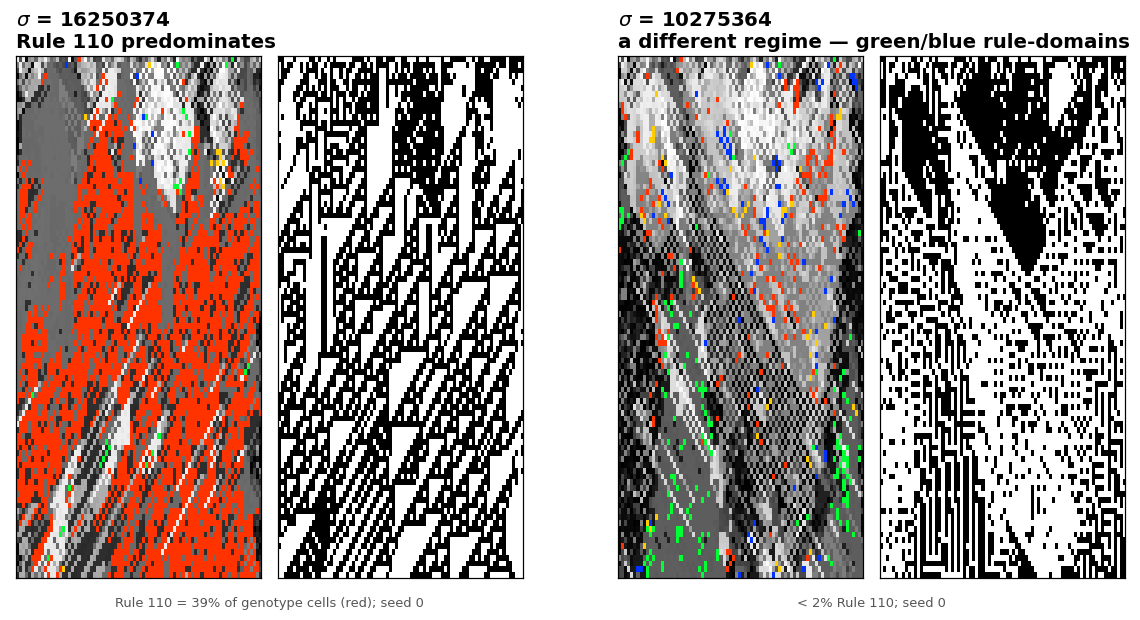
\includegraphics[width=\linewidth]{figures/rule110_spread.png}
\caption{Two operators from the family, each shown over time as genotype
(256-colour, left) and phenotype (black and white, right). Under
$\sig = 16250374$ the genotype field comes to be dominated by ECA
Rule~110---the red cells, $39\%$ of the genotype at the representative seed
($35\%$ over six seeds)---and the phenotype accordingly displays Rule~110's
characteristic gliders; under $\sig = 10275364$ a different regime of
rule-domains forms (green and blue, under $2\%$ Rule~110). The operator does not merely stir rule space: it
drives it toward particular, computationally distinguished rules. Genotype
colours are the legacy engine's own.}
\label{fig:regimes}
\end{figure}

\section{The Classification}
\label{sec:classification}

\subsection{Fixed points exist iff every cycle is even}

\begin{theorem}\label{thm:parity}
$P_\sig$ has a fixed point (a fixed rule) if and only if every cycle of
$\sig$ has even length. Since a one-cycle has odd length, this already
requires $\sig$ to be fixed-point-free.
\end{theorem}

\noindent A fixed rule is a $g$ invariant under~\eqref{eq:prop}, i.e.\ a
$\sig$-equivariant Boolean colouring with $g(\sig k) = \lnot\,g(k)$.
Follow a cycle of length $L$: equivariance forces
$g(k) = (\lnot)^{L} g(k)$, and $(\lnot)^{L}$ is the identity exactly when
$L$ is even; conversely, colour each orbit by the parity of its distance
from a chosen representative. A one-cycle of $\sig$ ($L=1$) is odd and so
admits no such colouring, which is why even cycles are required throughout.

Box~\ref{box:even-cycle} shows the theorem on the offset-$+2$ operator. The
same small calculation also makes the later $2^k$ count and forced
$\lambda=1/2$ balance visible before we state them generally.

\begin{workedexample}[label={box:even-cycle}]{Even and odd cycles}
\small
For offset $+2$ on eight truth-table positions,
\[
\sig=(0\;2\;4\;6)(1\;3\;5\;7).
\]
A fixed rule must change colour at every arrow because
$g(\sig k)=\lnot g(k)$. Around either four-cycle it can therefore read
$0101$ or $1010$: after four negations it returns consistently to its
starting bit. The two four-cycles are coloured independently, so two binary
choices fix all eight truth-table entries $\bit{0},\dots,\bit{7}$. Read back as
an ECA rule number---those eight bits in Wolfram neighbourhood order (the table
of \secref{sec:object}) taken as an integer in $0$--$255$---the four colourings
are the fixed rules
\[
2^2=4:\quad
51,\ 102,\ 153,\ 204,
\]
each with four zero-bits and four one-bits. An odd cycle admits no such
colouring: after an odd number of negations the bit returns to its starting
position demanding its own opposite, so no fixed rule exists. Admitting a fixed
rule and settling onto one are distinct. An operator carrying an odd cycle has no
fixed rule for its field to collapse onto, and its field correspondingly stays
diverse (the any-odd reduced rotate$+2$, Figure~\ref{fig:parity}, right); whether
a fixed-point-bearing operator collapses onto one of its fixed rules is a
separate, dynamical question (\secref{sec:interrupter}).
\end{workedexample}

This is the signed-cycle fixed-point theorem of Boolean-network theory
\parencite{aracena2008maximum} specialised to~\eqref{eq:prop}: our operator
is a Boolean network whose signed interaction digraph is $\sig$ with every
arc negative, a negation-cycle of length $\ell$ has sign $(-1)^\ell$, and
an isolated negative cycle admits no fixed point while a positive (even)
one admits exactly two. We contribute a machine-checked proof of the
specialised statement in Lean~4 / Mathlib.\footnote{%
\texttt{DarkTower/Patterns/Propagator.lean}, theorem
\texttt{hasAlternatingColouring\_iff\_cycleType\_even}; \texttt{lake build}
clean, no \texttt{sorry} or \texttt{axiom}.}

\subsection{The closed form}

The number of $\sig \in S_{2n}$ with all cycles even is $((2n-1)!!)^2$, with
exponential generating function $\sum_n ((2n-1)!!)^2 x^{2n}/(2n)! =
1/\sqrt{1-x^2}$ (the ``set of even cycles'' construction).
For $S_8$ this is $105^2 = 11{,}025$ of $40{,}320$, or $27.34\%$. The count
is classical: it is \textcite{oeis_a001818} and appears as
\textcite[Problem~5.34(c)]{stanley1999enumerative} and in
\textcite{riordan1968combinatorial}. We claim it only as the enumeration of
our operator family, not as a new identity.

\subsection{Fixed bytes number $2^k$}

\begin{corollary}\label{cor:count}
An all-even $\sig$ with $k$ cycles has exactly $2^k$ fixed bytes; any $\sig$ with
an odd cycle has none.
\end{corollary}
Each even cycle admits exactly two alternating colourings, chosen independently
across cycles, whence $2^k$; the zero case is Theorem~\ref{thm:parity}. This too
is machine-checked.%
\footnote{\texttt{alternatingColouring\_card\_eq\_two\_pow\_cycleType\_card}.}
Summed against these weights the family is consistent:
$\sum 2^{k}$ over all-even $\sig$ equals $(2n)! = 8! = 40{,}320$, the total
number of fixed bytes across the family.

\section{Every Fixed Point Is Balanced}
\label{sec:lambda}

\begin{definition}[Langton's activity $\lambda$]\label{def:lambda}
$\lambda$ measures a rule's \emph{activity}: the fraction of its neighbourhood
entries that map to the non-quiescent
state~\parencite{langton1990computation}---for an eight-bit ECA table, the
Hamming weight over eight, $\lambda = \lVert r \rVert_1 / 8$, from $0$ (every
neighbourhood dies) through $1/2$ to $1$. A rule with $\lambda = 1/2$ is
\emph{balanced}.
\end{definition}

\begin{observation}[label={obs:lambda}]{Balance is a truth-table property}
Langton's thesis was that complex behaviour concentrates near a critical
$\lambda$, shown most clearly for larger tables ($K=4$, $N=5$); for the
two-symbol, three-neighbour ECAs Langton is explicit that $\lambda$ only roughly
correlates with dynamics, and later work is
cautious~\parencite{mitchell1993revisiting}. Theorem~\ref{thm:lambda} below
concerns the \emph{value} $\lambda = 1/2$ itself---balance---which we keep
separate from any empirical claim about what it predicts dynamically.
\end{observation}

\subsection{Every fixed point has $\lambda = 1/2$}

\begin{theorem}\label{thm:lambda}
Every fixed point of every operator in the family has exactly four one-bits;
equivalently, Langton's activity parameter $\lambda = 4/8 = 1/2$.
\end{theorem}

\noindent By Theorem~\ref{thm:parity} each cycle has even length $2m$; an
alternating colouring assigns such a cycle exactly $m$ ones; summing over
cycles gives $(\sum L)/2 = 8/2 = 4$. Exhaustive enumeration confirms it:
across all $40{,}320$ operators and all their fixed points, every one has
Hamming weight four, with zero exceptions. The statement is machine-checked
for $\mathrm{Fin}\,8$.\footnote{%
\texttt{alternatingColouring\_true\_card\_eq\_four}: the true-cells and
false-cells are put in bijection by $\sig$, forcing each to number four.}

We are deliberate about the standing of this result. Langton's critical
value was obtained empirically, as a statistic over rule space
\parencite{langton1990computation}, and its status as an order parameter
was contested: \textcite{mitchell1993revisiting} refuted
\textcite{packard1988adaptation}'s specific genetic-algorithm clustering
claim, not the definition of $\lambda$, which survived as one axis among
others such as Wuensche's $Z$ \parencite{wuensche1999classifying}. There is
a folklore intuition for why $1/2$ is special --- binomial sampling variance
$\lambda(1-\lambda)$ is maximal there --- and it is not ours; and it has been
noted that $\lambda$ alone does not fix a rule's dynamical class, distinct
classes coexisting at a single value \parencite{sakai2002edge}. What
Theorem~\ref{thm:lambda} adds is narrower and firmer than any of these: under
the complementation in~\eqref{eq:prop} the value $1/2$ is \emph{forced} as an
algebraic matter, because any alternation-under-complement colouring is
balanced by parity. We claim balance, exactly; any connection of that
balance to dynamical behaviour we treat as interpretation, not as part of the
theorem.

\subsection{The cast: which rules survive, and how many}

Under an all-even $\sig$, the fixed points of $P_\sig$---the rules it maps to
themselves---number $2^k$, where $k$ is the number of cycles of $\sig$
(\secref{sec:classification}): each even cycle admits two alternating
colourings, chosen independently across cycles. In the spatial runs these are
the rules onto which the field is observed to settle. Every one has
$\lambda = 1/2$ (Theorem~\ref{thm:lambda}), so the observed terminal
population is a cast of \emph{distinct} rules---distinct truth tables---sharing
a \emph{single} activity.

The smallest nontrivial case of the count is a single cycle, $k = 1$: two
survivors. The 2015 paper's Figure~8 already exhibited a two-rule residual: a
random field of tens of distinct rules dies off to an alternating population of
just two, rules $42$ and $170$.
Fittingly, the programming error that produced the family is what pins its
residual at two---the erroneous mutation froze a bit, splitting the field
into the cells that can reach $42$ and those that can reach $170$---so the
phenomenon was on the page before the $2^k$ count explained it.

That die-off curve---the count of distinct rules present over time---is a
natural population-level companion to $\lambda$. Where $\lambda$ is a scalar
assigned to a single rule, this curve is a property of the whole field's
trajectory; and where $\lambda$ is uninformative here---every fixed point
sits at $1/2$---the curve still varies, because it measures the population
rather than the point. We use it cautiously, as an observable rather than an
established order parameter, to tell the rotations whose fields stay diverse
from those whose fields collapse (\secref{sec:interrupter},
Figure~\ref{fig:lambda}).

Diversity of the observed population and singularity of its activity thus
coexist; the metric measures we tried do not separate the two
(\secref{sec:metrics}).

\begin{figure}[t]
\centering

\includegraphics[width=\linewidth]{figures/fig2pair.png}
\caption{\textbf{Two terminal-diversity solutions of Figure~2's operator.} The
historical write $[0\,0\,1\,2\,3\,4\,5\,6]$ has two forms under the standard
Wolfram order. Its \emph{conjugate} $[1\,2\,4\,5\,3\,6\,7\,7]$ (top) reproduces the
draft3 behaviour: the genotype collapses to exactly two terminal rules---76 and 77,
adjacent, differing in a single bit---regardless of seed, while the phenotype stays
regular. Applied \emph{directly} (bottom), the same operator keeps a diverse
genotype (${\sim}30$ terminal rules)---the draft4 solution. Two ends of genotypic
aliveness from one historical write.}
\label{fig:fig2pair}
\end{figure}

\subsection{A dead genotype can carry a live phenotype}
\label{sec:shell}

The balanced shell is a definite object: exactly $\binom{8}{4} = 70$ rules
carry four active outputs, and by Theorem~\ref{thm:lambda} the absorbing set of
every operator in the family lies wholly inside it. Collapse is therefore not
merely a loss of diversity but a fall onto this particular $70$-rule shell---the
field dies \emph{onto the edge}, at $\lambda = 1/2$, always.

Balance is necessary for a genotype to freeze and silent about what the frozen
rule then does. Run each of the $70$ as an ordinary elementary CA and they
split: $32$ are phenotypically live---sustained change under iteration, the
additive rules $90$, $105$, $150$ and the class-IV rule $54$ among them---while
the rest fall quiescent. The two halves share a single $\lambda$; this is,
inside our family and by construction rather than by survey, the coexistence of
dynamical classes at one activity value that has long been urged against
$\lambda$ as an order parameter \parencite{sakai2002edge}. A field can thus die
in its genotype while the surviving rule keeps its phenotype in motion.

Figure~\ref{fig:shell} is such a field, built to specification. To seat a
collapse on a chosen live rule $R$ it suffices to pair $R$'s four active
positions with its four inactive ones as an involution: four transpositions, an
all-even operator that must collapse (Theorem~\ref{thm:parity}) and that holds
$R$ among its fixed points. Carried out for Rule~$54$ this yields
$\sig = [2\,3\,0\,1\,5\,4\,7\,6]$; run from a random field it drives the
genotype to near-uniformity---two rules survive---while the phenotype never
settles. The field has died onto Rule~$105$, another live tenant of the same
shell, whose additive dynamics keep the black-and-white panel full of
structure. Genotypic death and phenotypic death are not the same event.

One caveat marks the open edge of this. An involution fixes not its target
alone but the whole shell compatible with its pairing, and which tenant a
random field actually reaches is set by the basins, not by the construction: we
aimed at $54$ and the dynamics preferred $105$. Existence is settled---live
survivors are constructible---but \emph{steering} a field onto a named rule is
not, and is the natural next question.

\begin{figure}[t]
\centering
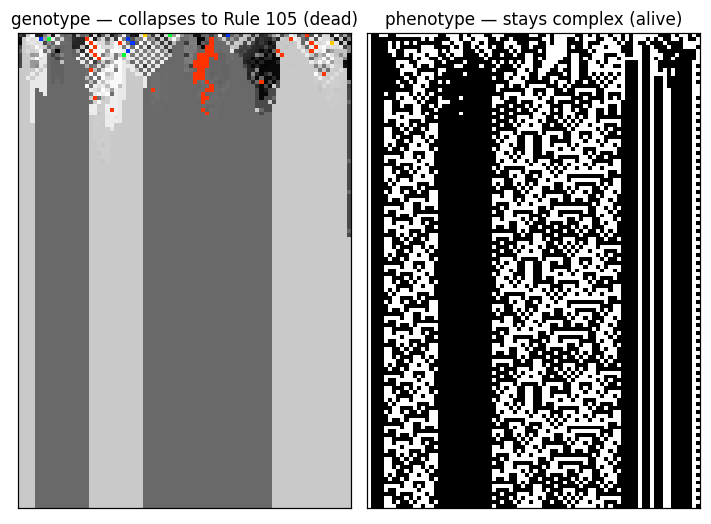
\includegraphics[width=0.82\linewidth]{figures/critical_shell.png}
\caption{A genotypically dead, phenotypically live field. The all-even operator
$\sig = [2\,3\,0\,1\,5\,4\,7\,6]$, built to fix the balanced shell containing
Rule~$105$, collapses the genotype (left, 256-colour) to near-uniformity within
a few dozen rows---two rules survive---yet the phenotype (right) never settles:
the field has died onto Rule~$105$, an additive $\lambda = 1/2$ rule whose
dynamics keep it complex. Seed~$1$, $W = 80$, $T = 120$.}
\label{fig:shell}
\end{figure}

\section{The Census}
\label{sec:census}

\subsection{The parity dichotomy in the spatial dynamics}

Theorems~\ref{thm:parity}--\ref{thm:lambda} concern fixed points; run as a
spatial dynamics, the parity dichotomy also shows in behaviour. Left to settle,
all-even operators collapse onto their fixed rules while any-odd operators stay
diverse (Figure~\ref{fig:parity}). The full census below
(\secref{sec:full-census}) makes this quantitative over all $40{,}320$ operators
(Table~\ref{tab:census}); the dynamical content is the \emph{death-rate
difference} between the classes, not the class sizes.

\begin{figure}[t]
\centering
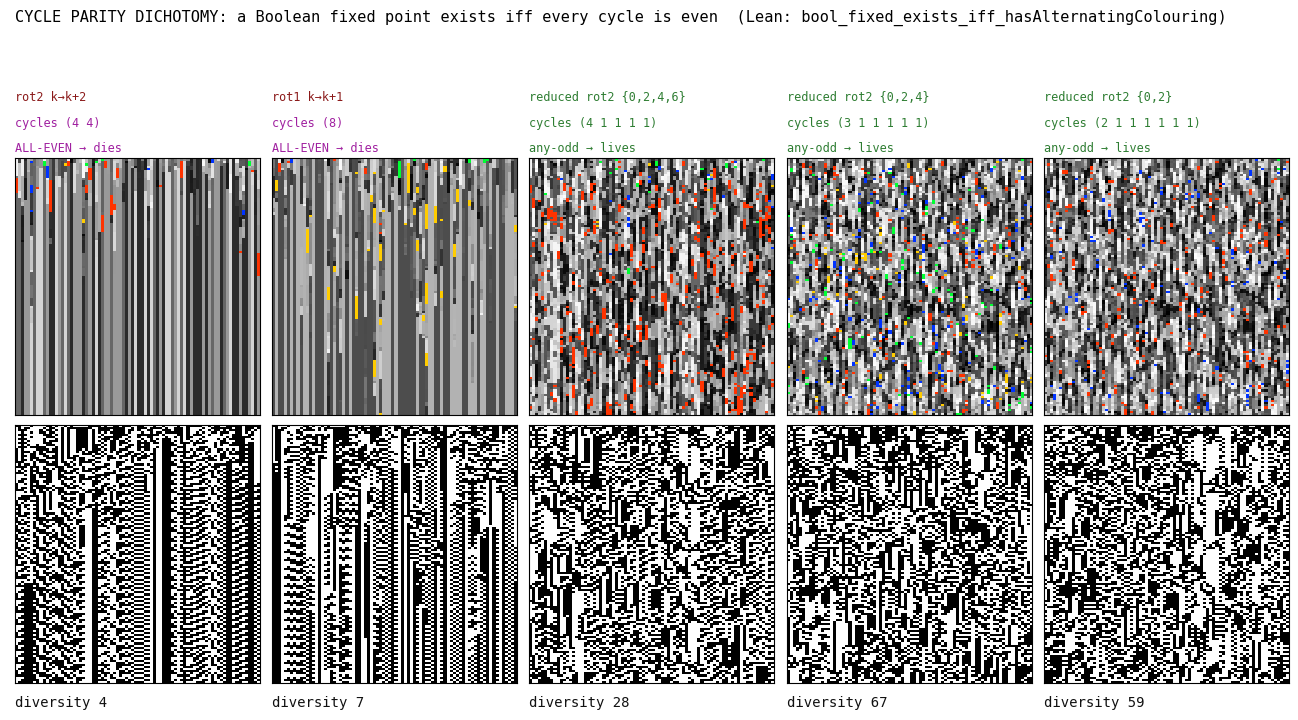
\includegraphics[width=\linewidth]{../../labs/M-aif-tokamak/compositions/parity-dichotomy.png}
\caption{The parity dichotomy, by example (the full census of $20{,}256$
orbits is summarised in the text). Five operators as genotype (top) and
phenotype (bottom) over time. \emph{Left:} the all-even operators
rotate$+2$ and rotate$+1$ possess fixed points (Theorem~\ref{thm:parity})
and, left to settle, the field collapses onto them---rotate$+2$ onto
four rules, its $2^k = 2^2$ count. \emph{Right:} the any-odd operators
(reduced rotate$+2$, acting on a subset so the remaining positions are odd
one-cycles) possess no fixed point, cannot settle, and stay diverse. This
settling is the operator left to itself; a neighbour-blend interrupter
reverses it for the $\gcd 2$ case (Figure~\ref{fig:lambda},
\secref{sec:interrupter}), and that reversal is the dynamical point.}
\label{fig:parity}
\end{figure}

\subsection{A prospective test: reduced rotate$+2$}

To guard against reading structure into a completed enumeration, we fixed a
prediction before running the case. The reduced $\text{rotate}{+}2$
operators act as a single even cycle on a subset of positions and leave the
remaining positions as one-cycles; by that leftover they are \emph{not}
all-even, so by Theorem~\ref{thm:parity} they possess no fixed point and
should fall on the no-fixed-points side of the dichotomy---no rule for the
field to settle onto, and correspondingly less extinction. They do
(Figure~\ref{fig:parity}, right): they stay diverse rather than dying off.
Absence of fixed points forbids settling onto a single rule; it does not
forbid short-period behaviour, and we claim only the observed persistence of
diversity, not literal aperiodicity.

\subsection{The full census, tabulated by class}
\label{sec:full-census}

\begin{definition}[Aliveness]\label{def:aliveness}
A layer is \emph{alive} on a run if its late-window \emph{change rate}---the mean
fraction of cells that differ between consecutive generations, over the last $40$
of the $100$ generations---is at least $0.10$; otherwise it is \emph{dead}.
Genotype and phenotype are scored separately (three seeds), giving four regimes:
live/live, live/dead, dead/live, dead/dead.
\end{definition}

The trend becomes a measured law once every operator is tabulated. We ran all
$40{,}320$ permutation-propagators and grouped them by cycle type
(Table~\ref{tab:census}).

\begin{expositionbox}{What the census shows}
\begin{pointbox}{Cycle parity draws the line, exactly}
Every cycle type with an \emph{odd} cycle is $100.0\%$ genotype-alive: having no
fixed rule (Theorem~\ref{thm:parity}), the field cannot collapse. Every
\emph{all-even} type splits---a fixed rule exists, but settling onto it is
dynamical.
\end{pointbox}
\begin{pointbox}{Collapse rises with the cycle count $k$}
Among all-even types the alive fraction falls as the cycles shorten: $[8]$
($k{=}1$) is $83\%$ alive, $[2\,6]$ and $[4\,4]$ ($k{=}2$) $70$/$67\%$, $[2\,2\,4]$
($k{=}3$) $49\%$, $[2\,2\,2\,2]$ ($k{=}4$) only $26\%$. This is the
$k$-dependence the qualitative run could only suggest.
\end{pointbox}
\begin{pointbox}{Most operators live; all four regimes are bijective}
$92.5\%$ have a live genotype. The $2\times2$ split is $82.7\%$ live/live,
$9.8\%$ live/dead, $6.0\%$ dead/dead, $1.4\%$ dead/live---so even Figure~2's
live/dead mirror is reached by $3{,}953$ \emph{permutations}, not only by the
non-bijective writings of Definition~\ref{def:writing}.
\end{pointbox}
\end{expositionbox}

\begin{table}[t]
\centering\small
\caption{Genotype-alive fraction by cycle type, over all $40{,}320$
permutations. Any odd cycle forbids a fixed rule and yields $100\%$ life
(Theorem~\ref{thm:parity}); the all-even types split, collapse rising with the
number of cycles $k$.}
\label{tab:census}
\begin{tabular}{lrr}
\toprule
cycle type & count & genotype-alive \\
\midrule
any type with an odd cycle (17 types) & $29{,}295$ & $100.0\%$ \\
$[8]$        & $5{,}040$ & $82.9\%$ \\
$[2\,6]$     & $3{,}360$ & $70.0\%$ \\
$[4\,4]$     & $1{,}260$ & $66.7\%$ \\
$[2\,2\,4]$  & $1{,}260$ & $49.2\%$ \\
$[2\,2\,2\,2]$ & $105$   & $25.7\%$ \\
\bottomrule
\end{tabular}
\end{table}

\section{Fixed Points Are Not Attractors}
\label{sec:interrupter}

\begin{figure}[p]
\centering
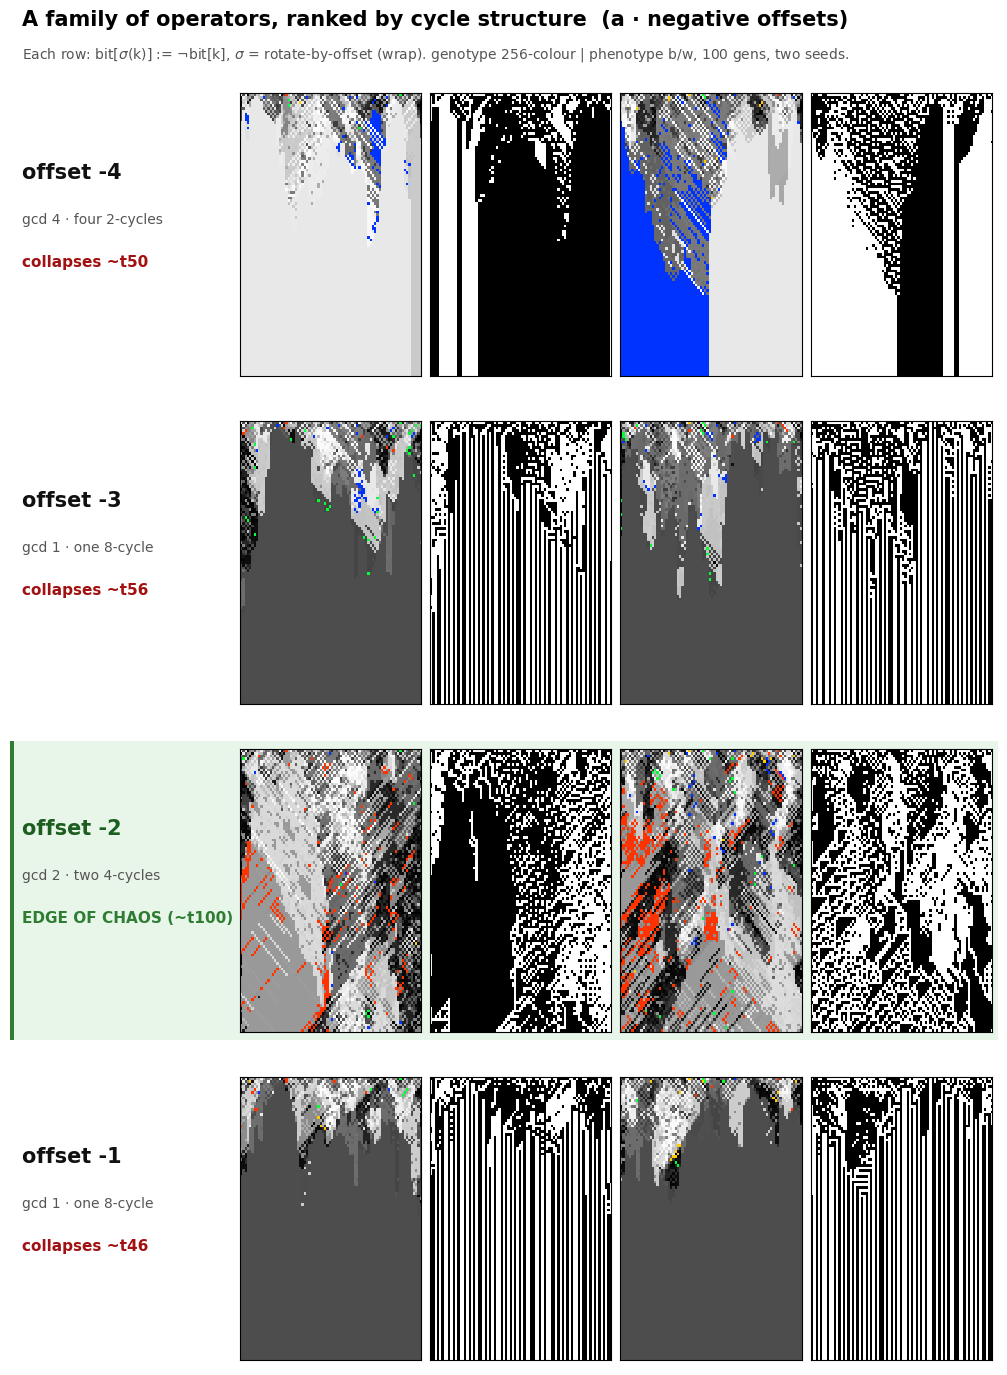
\includegraphics[height=0.90\textheight]{figures/survey_a.png}
\caption{\textbf{(a)~Negative offsets.} The rotation subfamily, ordered by
offset: each row is one wrap rotation $\bit{\sig(k)} := \lnot\,\bit{k}$ (two
seeds; genotype in 256 colours, phenotype black and white, first hundred
generations). Of these all-even rotations only the single 8-cycles,
$\gcd(\text{offset},8) = 1$---offset $\pm 1$ and $\pm 3$, highlighted---sustain a
high-diversity phase; offset $\pm 2$ ($\gcd 2$) and $\pm 4$ ($\gcd 4$) collapse.
See Worked Example~\ref{box:survey}; continued in~(b).}
\label{fig:eoc}
\end{figure}

\begin{figure}[p]
\ContinuedFloat
\centering
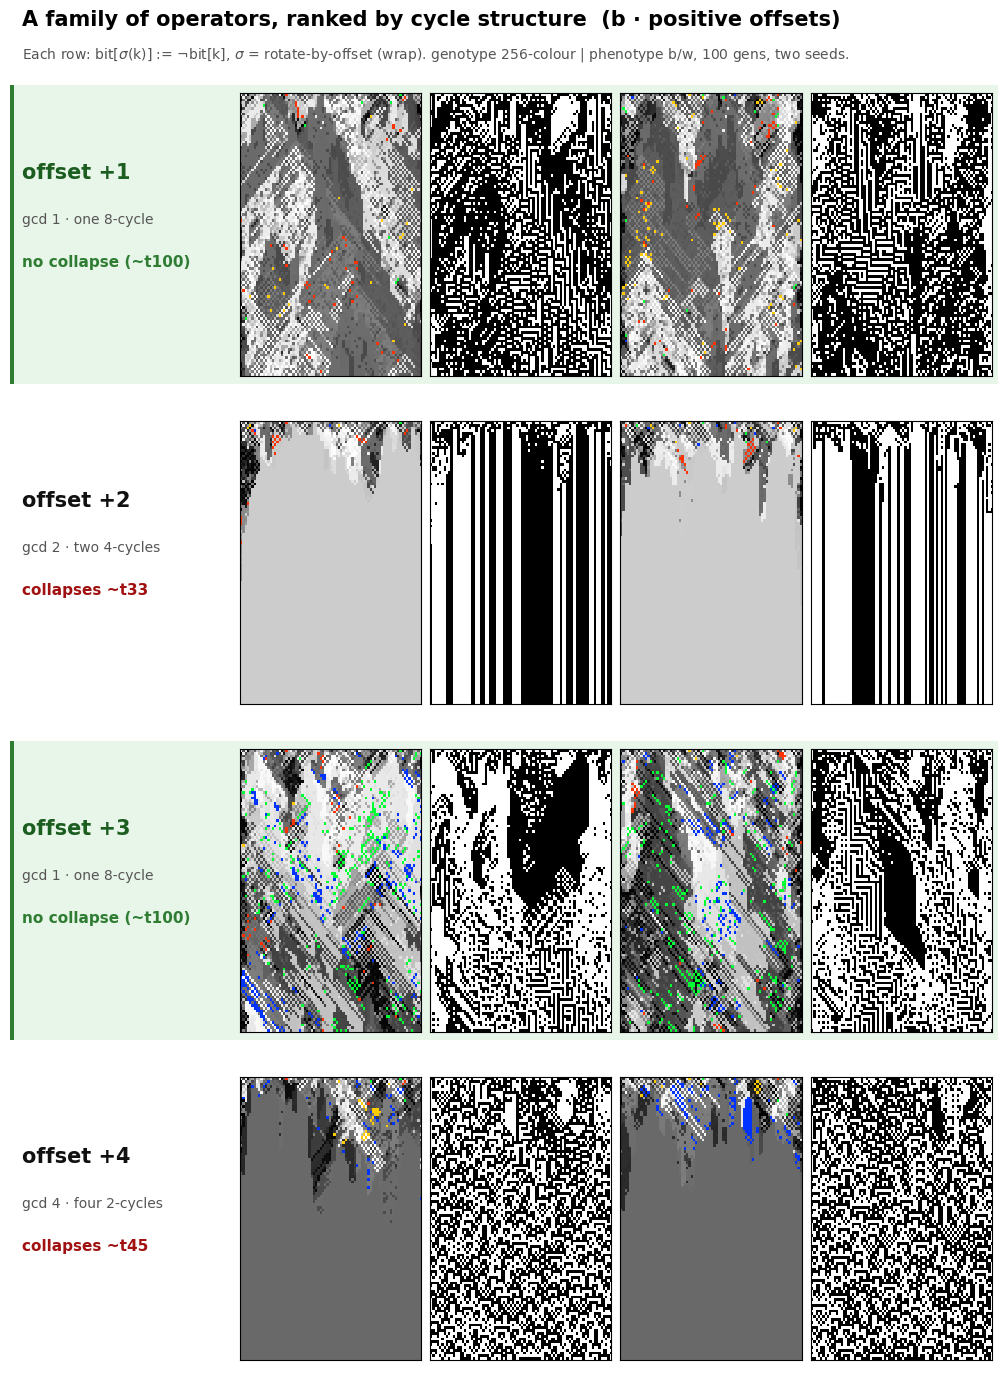
\includegraphics[height=0.90\textheight]{figures/survey_b.png}
\caption{\textbf{(b)~Positive offsets.} Continued from~(a). The classification is
symmetric under $d \to -d$ (verdict follows $\gcd(d,8)$), so offset $+1$ sustains
as offset $-1$ does, and offset $+2$ collapses as offset $-2$ does---inverse
rotations sharing verdict but not their transients (Worked
Example~\ref{box:survey}). Possessing a fixed point and staying near it are
different properties: this pair of pages is the whole paper in one figure.}
\end{figure}

\begin{workedexample}[label={box:survey},breakable=false]{Reading the rotation survey}
\small
The fields of Figure~\ref{fig:eoc} evolve under the \emph{spatially coupled}
dynamics of \secref{sec:interrupter}---the per-cell operator together with the
coupling between cells---not $P_\sig$ applied cell-by-cell. This is what the
survey turns on: under the bare operator every all-even rotation shown freezes
onto its fixed rules (Figure~\ref{fig:parity}, left). The coupling reverses this
for the single 8-cycles alone---$\gcd(\text{offset},8)=1$, offset $\pm 1$ and
$\pm 3$, fixed-point-bearing operators that nonetheless sustain a high-diversity
field---while offset $\pm 2$ ($\gcd 2$) and $\pm 4$ ($\gcd 4$) collapse
regardless; that split is what the survey shows.

The two panels are \emph{almost} mirror images, and where they differ is
instructive. Offset $+d$ and offset $-d$ are the same permutation exactly when
$2d \equiv 0 \pmod 8$---so offset $\pm 4$ (and the identity) are one operator with
bit-identical panels, whereas offset $\pm 1$ and $\pm 3$ are distinct
\emph{inverse} rotations. Inverses share cycle structure, fixed rules, and the
sustain-or-collapse verdict, but not their transient dynamics: offset $+1$ and
offset $-1$ realise the same sustaining regime through visibly different fields.
\end{workedexample}

Possessing a fixed point (Theorem~\ref{thm:parity}) is not the same as
reaching one, and $P_\sig$ does not by itself move a rule toward
$\lambda = 1/2$. Because $P_\sig$ complements every bit,
$\lambda(P_\sig g) = 1 - \lambda(g)$: the operator \emph{reflects} activity
across $1/2$, exactly preserving the distance $\lvert\lambda - 1/2\rvert$
rather than contracting toward it. And because $P_\sig$ is a bijection on
bytes, a generic rule lies on a periodic orbit and simply cycles---its fixed
points are fixed, but they are not attractors and have no basins. The only
rules pinned at $\lambda = 1/2$ are the fixed points themselves. Whatever
pull toward balance the \emph{spatial} field exhibits must therefore come
from the coupling between cells and from the interrupter below, not from the
bare map.

\begin{empiricalfinding}[label={find:survey}]{The rotation survey}
Every non-trivial wrap rotation is all-even and so possesses fixed rules
(Theorem~\ref{thm:parity}), yet in the spatially coupled dynamics they split by
cycle structure (Figures~\ref{fig:eoc},~\ref{fig:lambda}):
\begin{itemize}\setlength{\itemsep}{1pt}
\item the single 8-cycles---$\gcd(\text{offset},8)=1$, offset $\pm 1$ and
$\pm 3$---\emph{sustain} a high-diversity field, holding $\sim$30--40 distinct
rules through the longest runs we made ($400$ generations);
\item offset $\pm 2$ ($\gcd 2$, two $4$-cycles) and offset $\pm 4$ ($\gcd 4$,
four $2$-cycles) \emph{collapse} to one or two rules within a few dozen
generations.
\end{itemize}
The distinct-rule population curve (Figure~\ref{fig:lambda}) separates the two by
more than an order of magnitude in a single scalar. Possessing a fixed rule and
having the field stay near it are different properties; only the second is
visible in a drawing, and the interrupter (\secref{sec:interrupter}) is what
holds the 8-cycles off their fixed rules. We do not claim the count is an order
parameter in the statistical-mechanics sense; it is a summary of what the
drawings show, on the two seeds per operator that we ran.
\end{empiricalfinding}

\begin{figure}[t]
\centering
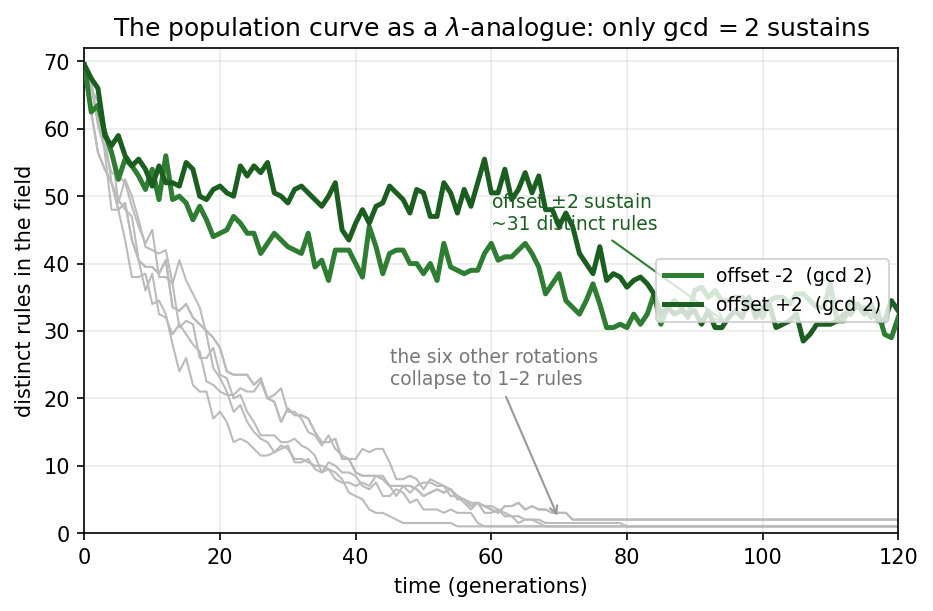
\includegraphics[width=\linewidth]{figures/lambda_analogue.png}
\caption{A population observable: distinct rules in the field over time, for
the wrap rotations (two seeds each). All begin at $\approx 70$; the four
8-cycles, $\gcd(\text{offset},8)=1$ (offset $\pm 1$ and $\pm 3$, green), keep a
large diverse population, while offset $\pm 2$ and $\pm 4$ (grey) collapse to one
or two rules. This makes quantitative, on the runs shown, the difference visible
by eye in Figure~\ref{fig:eoc}. The interrupting neighbour-blend is essential to
the sustained case: without it these same operators, in the census runs, instead
settle onto a handful of rules matching their $2^k$ count (the 8-cycles onto two,
offset$+2$ onto four; Figure~\ref{fig:parity}).}
\label{fig:lambda}
\end{figure}

\begin{figure}[t]
\centering
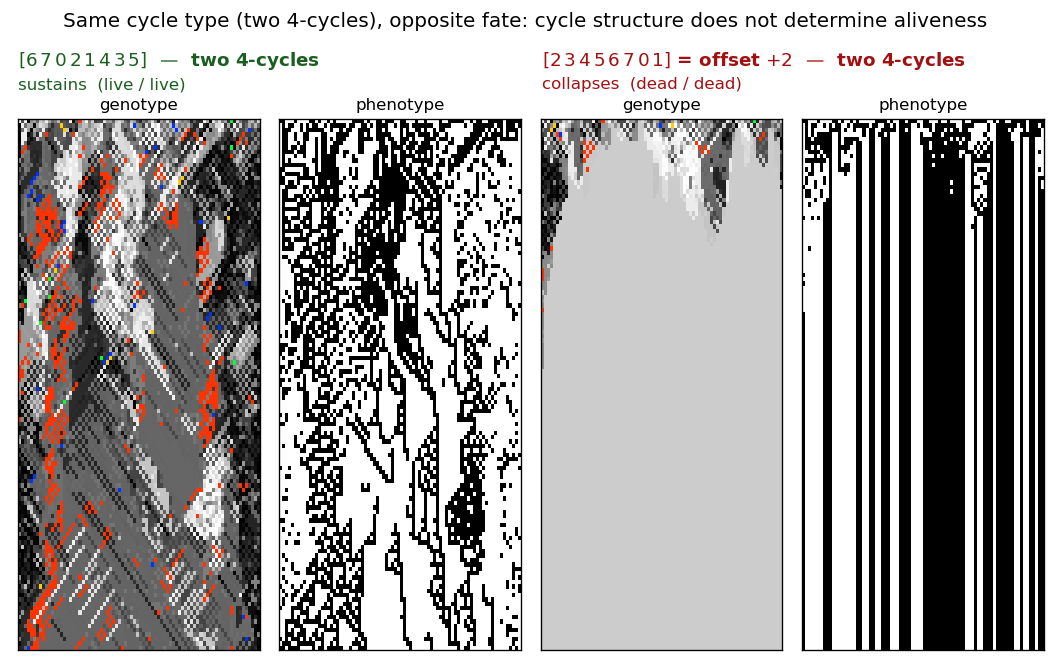
\includegraphics[width=\linewidth]{figures/two4cycle.png}
\caption{\textbf{Cycle structure does not determine aliveness.} Two operators of
identical cycle type---both two 4-cycles---with opposite fate. Left,
$[6\,7\,0\,2\,1\,4\,3\,5]$ sustains a live genotype and phenotype; it is the
standard-Wolfram-order form of the operator draft3 called offset$+2$ (its
conjugate). Right, the Wolfram-order rotation offset$+2=[2\,3\,4\,5\,6\,7\,0\,1]$
has the same two-4-cycle structure yet collapses to a dead genotype and a frozen
phenotype. Same cycle type, opposite outcome: the specific permutation, not its
cycle type alone, decides. A full census of the 40320 operators confirms the
two-4-cycle class splits between sustaining and collapsing.}
\label{fig:two4cycle}
\end{figure}

\begin{figure}[t]
\centering
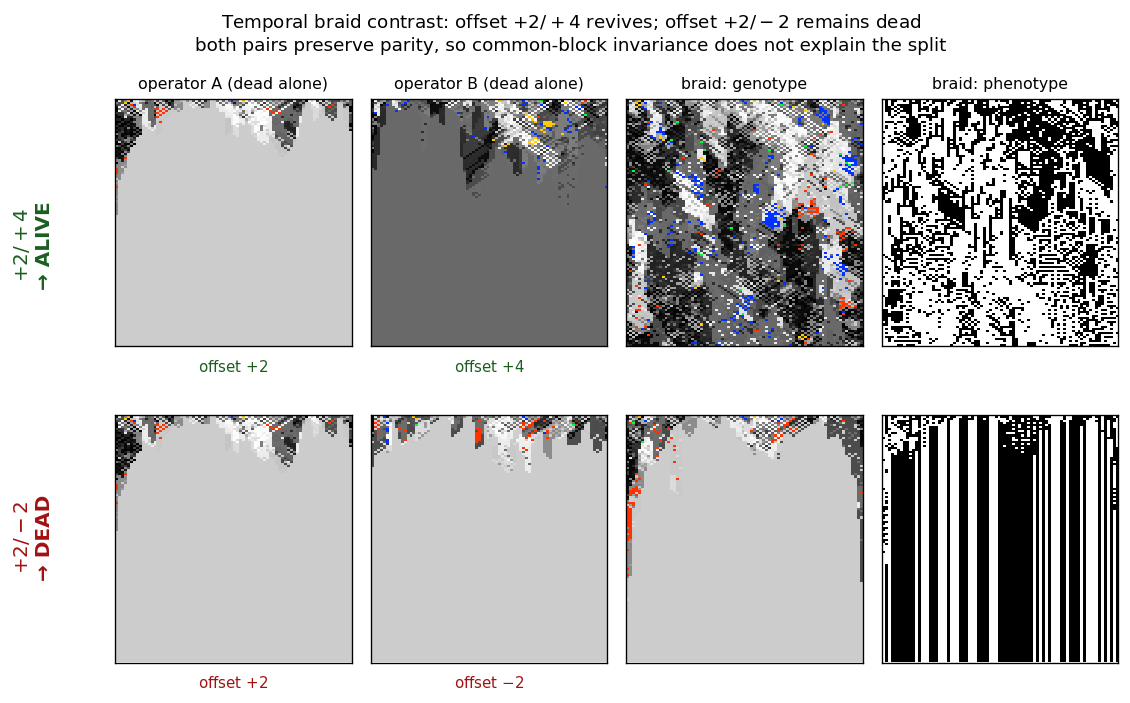
\includegraphics[width=\linewidth]{figures/braid.png}
\caption{\textbf{Braiding manufactures aliveness.} Two operators that each collapse
alone can be \emph{braided}---alternated step by step---into a sustained field, but
only when they preserve \emph{different} block systems. Top: offset$+2$ (two
4-cycles) and offset$+4$ (four 2-cycles) are each genotypically dead, yet their
braid is alive (genotype change-rate $0.76$, vs.\ $0$ for either alone). Bottom:
offset$+2$ braided with offset$-2$ stays dead---both preserve the same evens/odds
partition, so the alternation never leaves it. Composition is thus a constructive
tool: complementary dead operators synthesise an edge-of-chaos braid.}
\label{fig:braid}
\end{figure}

\begin{figure}[t]
\centering
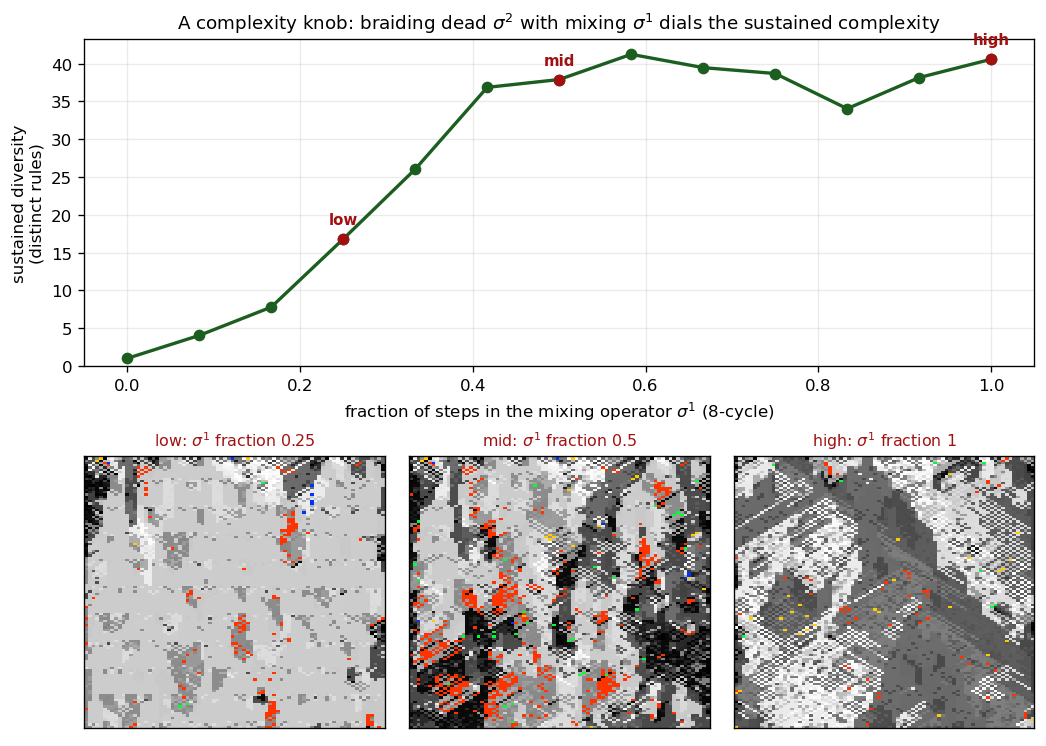
\includegraphics[width=\linewidth]{figures/knob.png}
\caption{\textbf{A complexity knob.} The powers of an 8-cycle
$\sigma$ form a lattice of block systems---$\sigma^1$ (no invariant partition,
maximal mixing), $\sigma^2$ (two 4-cycles), $\sigma^4$ (four 2-cycles)---with the
\emph{intermediate} powers dead and the ends alive. Braiding the dead $\sigma^2$
with the mixing $\sigma^1$, the sustained diversity is set by the fraction of steps
spent in $\sigma^1$: it climbs from dead ($\sigma^1$ fraction $0$) to saturation
(fraction ${\gtrsim}0.4$). The three panels show the field thickening from sparse
(low) to full edge-of-chaos (high) as the knob is turned---the same two operators
throughout, only the schedule changing. Composition is thus not just constructive
but \emph{tunable}: a super-propagator that controls its own complexity.}
\label{fig:knob}
\end{figure}

\begin{definition}[Interrupter]\label{def:interrupter}
An \emph{interrupter} is a step that occasionally declines to propagate---a
neighbour-blend that copies where neighbours agree, or a hold-when-active gate.
Composed with the operator, the coupled dynamics no longer settles: instead of a
frozen byte or a runaway cycle, the field holds a diverse population of rules,
many at $\lambda = 1/2$. The coordinate-wise blend of Box~\ref{box:metaca-step}
is the interrupter used in the ordinary spatial runs.
\end{definition}

\begin{observation}[label={obs:couplings}]{Two couplings of one operator}
This resolves the apparent tension between the census and
Figure~\ref{fig:lambda}: they are the same operator under two \emph{couplings}.
Left to settle, the field under rotate$+2$ collapses onto a few of its fixed
points; with the interrupter it is held off them and keeps tens of rules.
Settling and sustained diversity are two behaviours of one operator, selected
not by the bare algebra but by the coupling.
\end{observation}

\begin{observation}[label={obs:flat}]{The family is flat under its own composition}
Each operator of Equation~\eqref{eq:prop} negates every bit
($P_\sig(g)[j] = \lnot\,g[\sig^{-1}(j)]$, a coordinate permutation followed by a
global flip), so under composition the flips cancel in pairs: $P_\sig \circ
P_\tau$ is a \emph{pure} coordinate permutation with no negation left---a
bijection that fixes $2^{c}$ bytes for $c$ cycles but carries none of the forced
$\lambda = 1/2$ structure. An even number of propagators composes to such a bare
permutation, an odd number back to a single propagator; either way the composite
contains nothing the individual operators did not. We searched composites of two
and three operators for emergent structure and found none---the negation that
gives one operator its balanced fixed point is exactly what a second cancels.
\end{observation}

Propagators thus do not compose usefully with one another; the compositions that
\emph{do} yield something new must pair a propagator with a step of a different
kind.

One such composition is worth exhibiting.

\begin{definition}[River]\label{def:river}
A \emph{river} is the composed operator obtained by following the collapsing
offset-$+2$ propagator ($\gcd 2$) with a phenotype-reading construction
step---match the local phenotype against four template candidates, first match
wins, falling back to the all-zero rule---yielding a coherent band of
alternating phenotype that drifts through a disordered background and reappears
in all six seeds we tried (Figure~\ref{fig:river}).
\end{definition}

Where the bare rotation collapses or cycles, this
composition holds an off-critical structure for the length of every
run---its trajectory varying with the seed, its presence not. We report these
two mechanisms here; a fuller catalogue of composed operators is future work.

\begin{figure}[t]
\centering
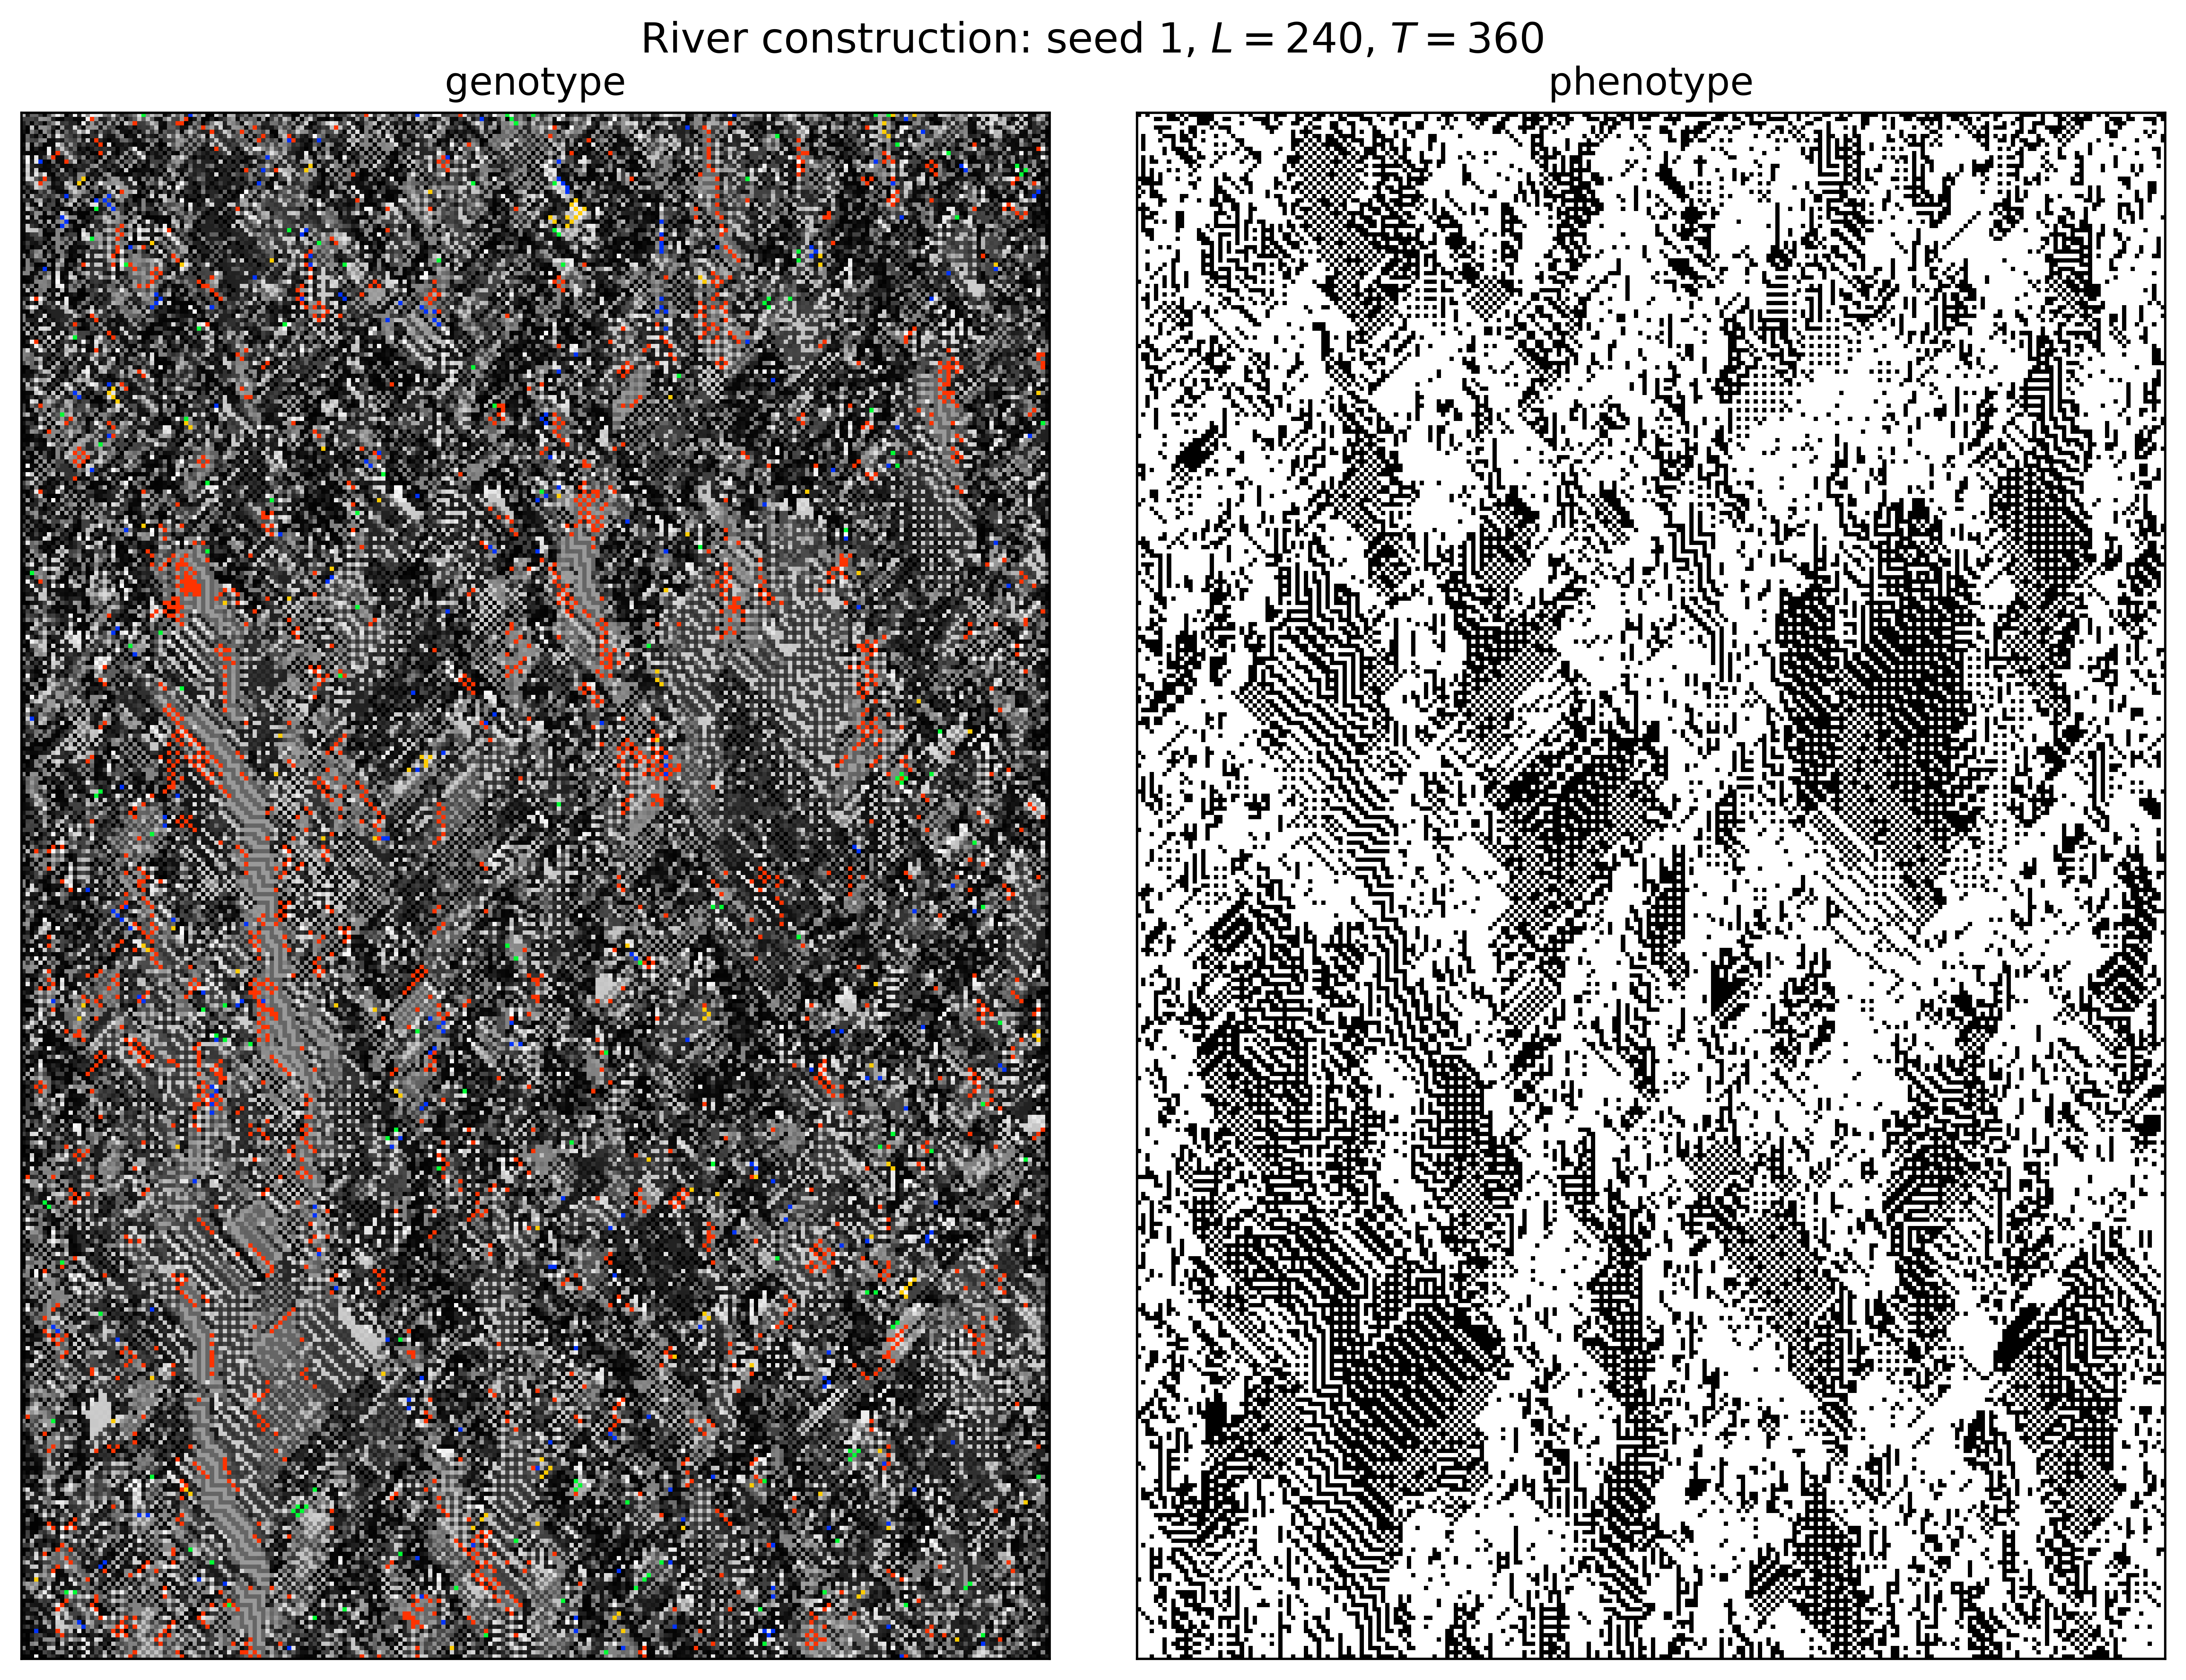
\includegraphics[width=\linewidth]{figures/river.png}
\caption{A \emph{river}: a composed operator sustains a reproducible
structure. The offset-$+2$ propagator, composed with a phenotype-reading,
four-candidate, first-match template construction (fallback: the all-zero
rule), produces in
each of six seeds a coherent band of alternating phenotype (bottom row)
drifting through a disordered background (genotype top, six seeds; genotype
coloured by rule as in Figures~\ref{fig:regimes}--\ref{fig:eoc}---greyscale by
byte value, with well-known ECAs highlighted, red~$=$~Rule~110). The band's
trajectory varies with the seed; its presence does not.
Where the bare rotations collapse or cycle (Figure~\ref{fig:eoc}), this
composition holds an off-critical structure for the length of the run.}
\label{fig:river}
\end{figure}

\section{Why Distance Geometry Cannot See This}
\label{sec:metrics}

\begin{observation}[label={obs:metrics}]{Why per-trajectory metrics cannot see the classification}
The classification is a conjugacy invariant of $\sig$---its cycle type---while
the complexity and compression measures we tried read a single rule's bits or one
space--time trajectory. A quantity read off one field's history has no access to
$\sig$'s cycle type, so it cannot recover the parity classification, and in our
tests it did not: a population count reads a collapsed-but-maximally-selected
field as nearly dead; a frozen periodic genotype scores a lower statistical
complexity $C_\mu$ \parencite{crutchfield1989inferring} than Rule~110; gzip rates
a self-similar rule as noise. We claim no general impossibility theorem---only
that the standard per-trajectory measures we tried do not separate the parity
classes, unsurprisingly, because the classifying property lives on the operator,
not on the states. The classification is a theorem \emph{because} it is not a
per-trajectory statistic.
\end{observation}

\section{Discussion}
\label{sec:discussion}

\begin{expositionbox}{Is the surviving phase a critical point? We test and ask a sharper question}
The survey (Figure~\ref{fig:eoc}) exposes a sharp behavioural split within a
family of provably fixed-point-bearing operators: only the single 8-cycles
(offset $\pm 1$, $\pm 3$) sustain a high-diversity phase, while offset $\pm 2$ and
$\pm 4$ collapse. A reader is entitled to ask whether that phase sits at a
\emph{critical point}---tuned between an ordered and a disordered phase, as CA
complexity is often supposed to \parencite{langton1990computation}. We test this
directly with a finite-size scan and find no such point, so we ask a different,
answerable question: whether the sustained diversity is spatially organised into
coexisting dynamical regimes.
\end{expositionbox}

\begin{empiricalfinding}[label={find:crossover}]{No critical point: a drifting susceptibility peak, read as metastability}
The natural control parameter is the \emph{propagator fraction} $q$ ($q = 0$ all
blend, $q = 1$ all propagator, offset $+1$). Across widths $L = 30$--$240$ (32
seeds each) the genotype activity $a_G(q)$ rises \emph{smoothly}, well described
by a logistic crossover ($R^2 > 0.99$, Figure~\ref{fig:phase}a); its width does
not shrink with size ($w \approx 0.13$, $w \sim L^{-0.04}$), so the curve never
steepens into the step a genuine transition would. The size-scaled run-to-run
spread $L\,\mathrm{Var}(a_G)$ (Figure~\ref{fig:phase}b) is a susceptibility: it
\emph{peaks} inside the crossover band, but the peak drifts in location
($q \approx 0.15$--$0.5$ across $L$) and grows only ${\sim}1.1\times$ from the
smallest width to the largest---failing the convergence-and-growth test a
critical point requires. At $q = 1$, the pure-propagator limit at which offset
$+1$ runs, the spread is instead \emph{low}: the field reliably organises into
\emph{system-spanning domains} (Figure~\ref{fig:tint}), reproducibly rather than
through a fluctuating transition. The honest reading is \emph{metastability}, not
criticality---seed-dependent residence times dominate this horizon, and we claim
no confirmed critical point.
\end{empiricalfinding}

\begin{empiricalfinding}[label={find:littoral}]{A finite-width littoral edge, not a phase boundary}
An intermediate-activity band ($0.15 \le a_G \le 0.60$) has a \emph{lower} edge
robustly at $q \approx 0.1$---stable under both system size and threshold---while
its upper edge is threshold-dependent, because $a_G$ saturates gradually rather
than jumping (the band spans $q \approx 0.1$ to $0.4$--$0.5$). This finite-width
crossover is best read as a \emph{littoral edge}: a shore of finite width rather
than a thermodynamic phase boundary. Where the bare rotations collapse or cycle
(Figure~\ref{fig:eoc}), offset $+2$ holds it for the length of the run.
\end{empiricalfinding}

\begin{definition}[Isolated-rule activity score]\label{def:activity}
The \emph{activity score} of a rule is its asymptotic per-step cell-change rate
when run alone as an elementary CA from a random initial condition---a run-time
measure, distinct from the static truth-table balance $\lambda$
(\secref{sec:lambda}). Ordered rules score near $0$; activity rises through the
complex rules (Rule~$110 \approx 0.4$) to the chaotic ones ($\gtrsim 0.5$). The
score \emph{orders} the regimes but does not by itself separate complex from
chaotic.
\end{definition}

Tinting the genotype by this score (Figure~\ref{fig:tint}) resolves the
intermediate field into coexisting low- and high-activity domains whose
boundaries trace filamentary sets through $1{+}1$-dimensional spacetime---objects
\emph{analogous to} the domain boundaries of computational mechanics
\parencite{crutchfield1989inferring,shalizi2001computational}, here obtained by
thresholding a scalar tint rather than by predictive equivalence.

\begin{empiricalfinding}[label={find:walls}]{The fractal domain walls are where the genotype is rewritten fastest}
The activity field resolves into ordered and chaotic domains separated by
\emph{fractal-like walls} (Figure~\ref{fig:interface}; box-counting dimension
$D \approx 1.5$--$1.7$ over $L = 128$--$768$, a handful of seeds). Those walls are
the locus of maximal \emph{genotypic} change: measuring the row-to-row rewrite
rate by region (Table~\ref{tab:churn}), the wall churns more than either
interior---for offset $+2$ at $L = 256$, $0.83$ at the wall against $0.77$
(ordered) and $0.58$ (chaotic)---and exceeds \emph{both} interiors in every one of
the $32$ committed operator/width/seed fields (offset $+2$, the river, $\sigma =
16250374$). The chaotic domain is in aggregate the most \emph{genotype}-stable, so
the wall---where ordered abuts chaotic---is where the propagator does its most
rewriting. The walls are not compositionally special (no rule class enriched;
Rule~110 if anything depleted), so the distinction is dynamical, not chemical.
Whether that rewriting transports or combines information \emph{along} the walls
we do not test---the natural question for a sequel.
\end{empiricalfinding}

\begin{expositionbox}{What we do not claim}
Two stronger claims are deliberately withheld. We do not assert a critical
transition---the scan is a null result, and the interface analysis is exploratory
(few seeds; the fixed-boundary line variant rather than the wrapped lattice of
Figure~\ref{fig:eoc}). Nor do we claim computation: held-out injection--decode
tests validate genotype storage and limited transmission in the feedforward
system, but under the river treatment the matched feedback contrast shows little
capacity under these probes and no detectable XOR-like modification---and failure
of these probes is not itself evidence of no computation. The denser river
boundary ($D \approx 1.7$ versus $1.5$) is an \emph{unmatched} comparison and does
not establish that the genotype--phenotype coupling causes the difference.
\end{expositionbox}

\begin{expositionbox}{The sequel: do the filaments carry computation?}
If the filaments are domain boundaries they are candidate \emph{wires}. The
natural question is not which rules compose them---in our data the complex rules
are not enriched there---but whether information is \emph{transported along} them
and \emph{combined where they collide} \parencite{mitchell1993revisiting}.
Whether computation flows down the littoral filaments of these diagrams is a
question for another paper.
\end{expositionbox}

\begin{figure}[tb]
\centering
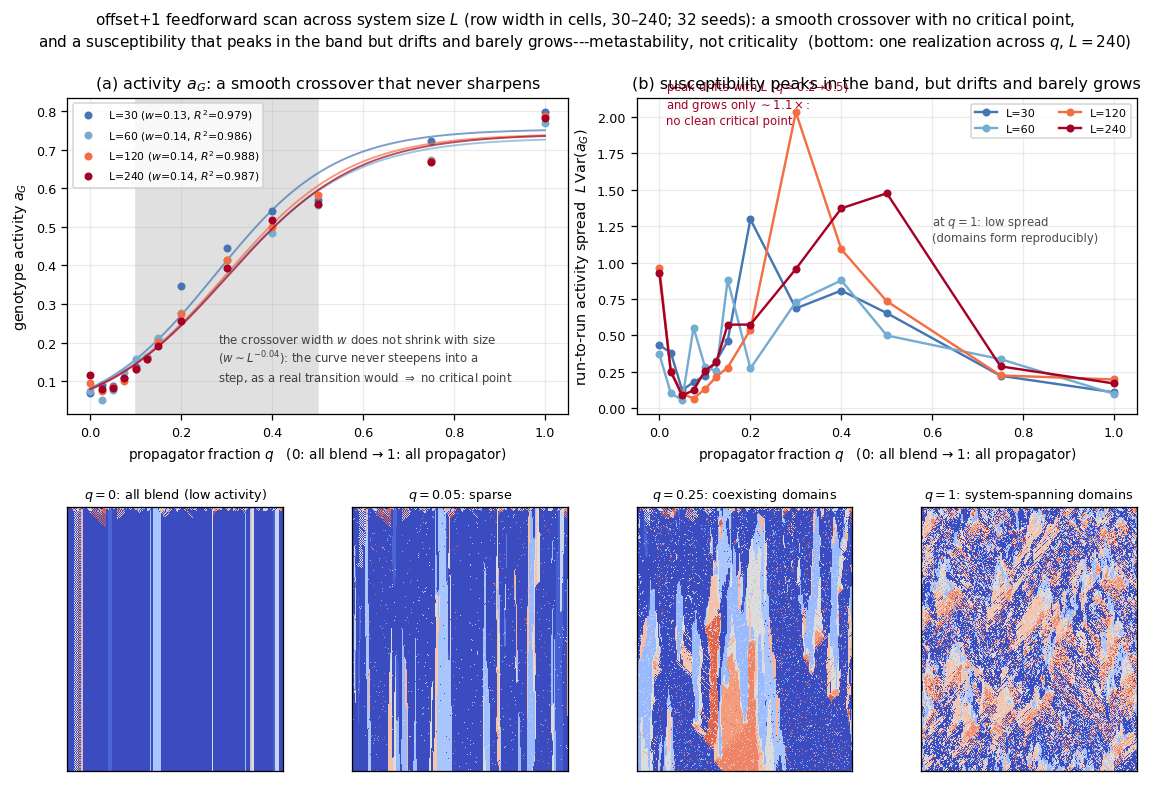
\includegraphics[width=\linewidth]{figures/eoc_phase.png}
\caption{\textbf{No critical point: the susceptibility peaks in the band but
drifts and barely grows.} offset $+1$ feedforward finite-size scan against the
propagator fraction $q$ ($0$: all blend, $1$: all propagator). $L$ is the
\emph{system size}---the lattice width in cells; the scan spans $L = 30$--$240$
(32 seeds each), because a genuine transition sharpens as $L$ grows while a
crossover does not. \textbf{(a)}~genotype activity $a_G$ with logistic fits
($R^2 > 0.99$); the crossover width is size-independent ($w \sim L^{-0.04}$), so
the curve never sharpens into a transition. \textbf{(b)}~the size-scaled
run-to-run spread $L\,\mathrm{Var}(a_G)$ is a susceptibility: it peaks inside the
band, but the peak drifts ($q \approx 0.15$--$0.5$ across $L$) and grows only
${\sim}1.1\times$, failing the convergence-and-growth test a critical point
requires; at $q = 1$ the spread is low, the field forming system-spanning domains
reproducibly. The honest reading is metastability, not criticality. Bottom: one
realisation ($L = 240$, single seed) tinted by isolated-rule activity, from
all-blend ($q=0$) to the pure-propagator limit ($q=1$).}
\label{fig:phase}
\end{figure}

\begin{figure}[tb]
\centering
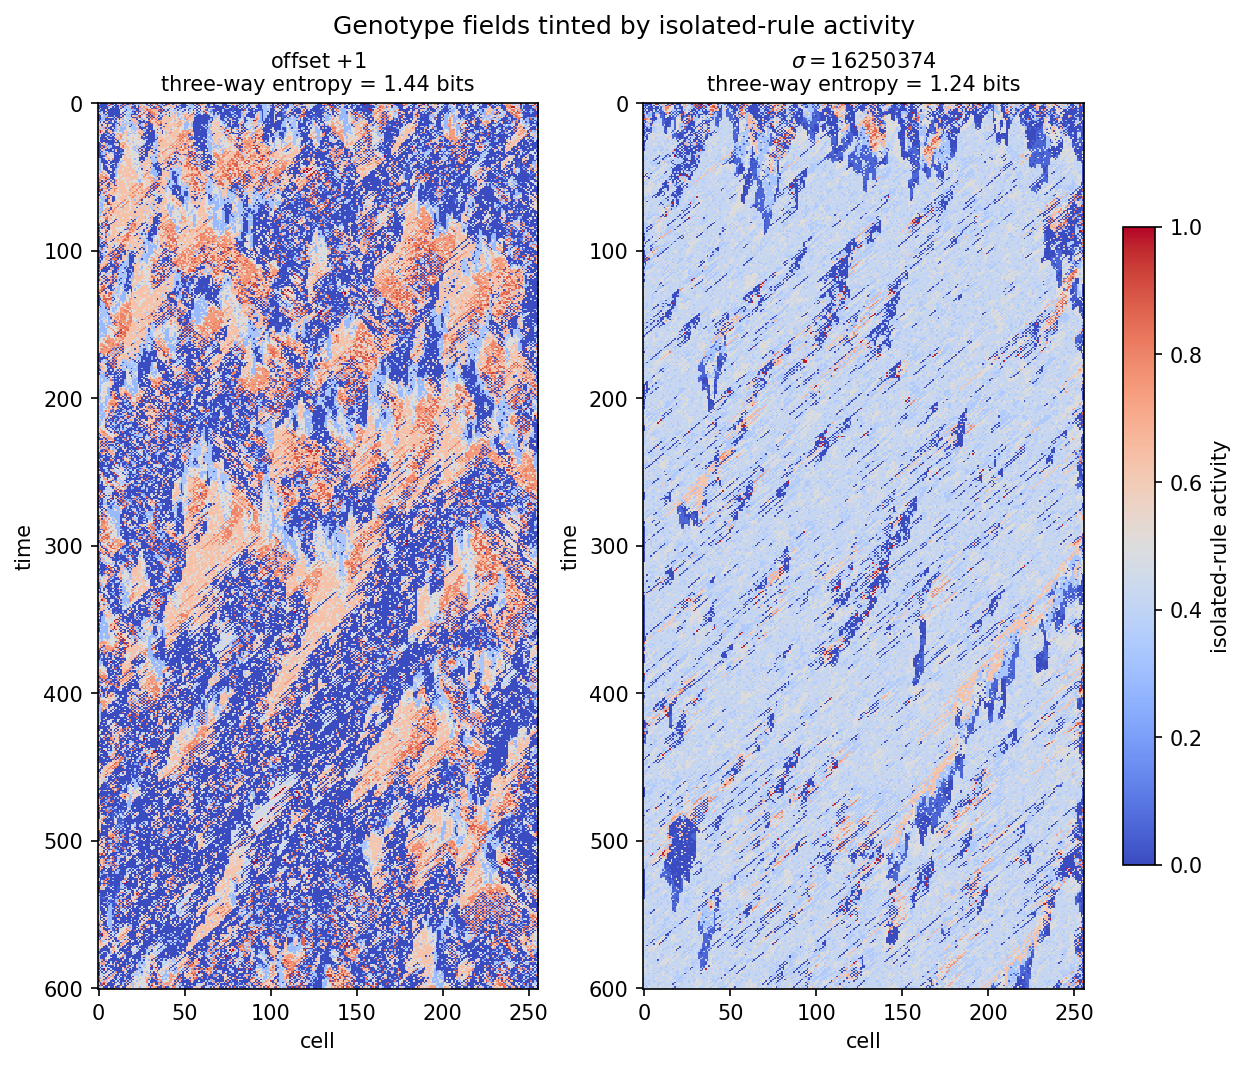
\includegraphics[width=0.68\linewidth]{figures/eoc_tint.png}
\caption{\textbf{The genotype as a map of activity regimes.} Genotype spacetime
fields (fixed-boundary variant) tinted by each rule's \emph{isolated-rule
activity score} (blue $=$ low near $0$, pale $=$ intermediate near $0.4$,
red $=$ high near $0.5$ and above). The field resolves into coexisting regimes,
and which active regime pairs with the low-activity background depends on the
operator: offset $+2$ mixes low activity with genuinely high-activity (chaotic)
rules ($\approx 40\%$ high at this seed), whereas $\sigma = 16250374$ is
dominated by the intermediate complex Rule~110 ($\approx 45\%$ at this seed).
The score orders the regimes but does not by
itself separate complex from chaotic, a known-hard distinction.}
\label{fig:tint}
\end{figure}

\begin{figure}[tb]
\centering
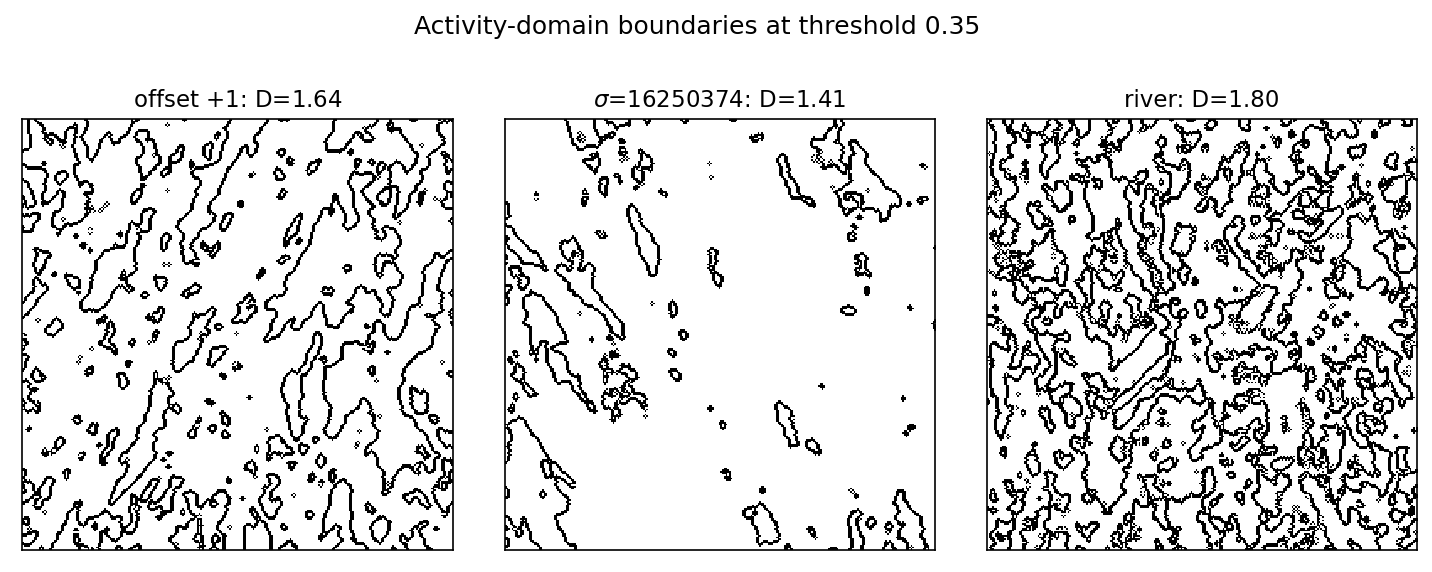
\includegraphics[width=\linewidth]{figures/eoc_interface.png}
\caption{\textbf{Activity-domain walls.} The boundary (black) between low- and
high-activity regions, traced through the $1{+}1$-dimensional spacetime diagram at
$L = 256$. offset $+2$ and $\sigma = 16250374$ carry fractal-like boundaries of
comparable interface fraction and dimension ($D \approx 1.5$--$1.6$); the
phenotype-coupled river carries a denser one ($D \approx 1.71$, an unmatched
comparison as it couples phenotype). The dimension is stable across
$L = 128$--$768$ (offset $+2$ and $\sigma \approx 1.5$, river $\approx 1.7$; box
sizes $2$--$64$). Collapsed operators (e.g.\ offset $+4$) carry none. These walls
are also where the rule field is rewritten fastest (Discussion). Exploratory: a
handful of seeds, fixed-boundary variant.}
\label{fig:interface}
\end{figure}

\begin{table}[tb]
\centering
\caption{\textbf{Genotype churn by region}---row-to-row rewrite rate of the rule
field (fraction of cells whose ECA rule changes from the row above), at
$L = 256$, mean over the committed seeds. For every operator the wall exceeds
\emph{both} domain interiors; the chaotic interior---most active in
phenotype---is the most genotype-stable. Wall extraction is the
threshold-and-smooth procedure of Figure~\ref{fig:interface}; reproducible from
the committed fields (\texttt{plot\_eoc\_churn.py}).}
\label{tab:churn}
\begin{tabular}{lccc}
\toprule
Operator & Wall & Ordered interior & Chaotic interior \\
\midrule
offset $+2$          & $0.83$ & $0.77$ & $0.58$ \\
$\sigma = 16250374$  & $0.71$ & $0.68$ & $0.57$ \\
river                & $0.98$ & $0.97$ & $0.88$ \\
\bottomrule
\end{tabular}
\end{table}

\section{Limits}
\label{sec:limits}

The theorems are the Boolean case and are exact; the dynamical claims are
narrower and empirical. The census and the sustained-diversity behaviour are
reported for a single spatial coupling ($S_8$, radius one, one value map) at
limited seed counts, and invite a fuller treatment. \secref{sec:discussion}
takes up the local, structural reading and reports an exploratory
interface-dimension statistic under its own stated caveats (few seeds,
fixed-boundary variant); beyond it we report no perturbation-spreading or
entropy-rate statistics.
Because the dynamics is stochastic, every such figure is given both as a
fixed \emph{representative} seed and, where a scalar is quoted, as a fixed
\emph{six-seed sample} (mean and range); both are reproducible from the
pinned seeds through the accompanying package. The
substrate the object sits in is not itself new (\secref{sec:object}); $\lambda$
is one heuristic among several \parencite{wuensche1999classifying}, and we
make no claim that balance implies any particular dynamics---only that here
balance is \emph{derived}. What is new, and what we rest the paper on, is the
object of Equation~\eqref{eq:prop} and the fixed-point structure that forces
every fixed rule to be balanced, $\lambda = 1/2$, as a matter of proof.

\section{Conclusion}
\label{sec:conclusion}

The characterisation promised at the outset (\secref{sec:object}) has two
halves. The
first is static and exact: which operators possess fixed points (the
all-even ones), how many ($2^k$), and where they lie (balanced,
$\lambda = 1/2$, always). The second is empirical and tentative. Because
every fixed point sits at $\lambda = 1/2$, that parameter is silent on the
difference between an operator whose field stays diverse and one whose field
collapses; the distinct-rule count is not, and in our
runs it separates the two across the rotation family by more than an order of
magnitude (Figure~\ref{fig:lambda}). The same observable offers a suggestive
reading of the search that produced the family, reported both as a
representative run and as a fixed six-seed sample (\secref{sec:limits}). The
operator of Figure~\ref{fig:regimes} that comes to be dominated by
Rule~110---a universal rule, the naive prize of a search for computational
intelligence---concentrates the field onto it and pays for it in diversity.
At the representative seed, $39\%$ of its genotype cells are Rule~110 and it
sustains $16$ distinct rules, against a foil that holds Rule~110 below $1\%$
and sustains $33$; over the six-seed sample the ordering is unchanged---Rule
110 $35\%$ (range $31$--$39\%$) versus $0.2\%$ ($0$--$0.2\%$), sustained diversity
$15$ versus $23$. On this pair, recovering a universal rule and sustaining a
diverse population pull against each other---a suggestion worth testing at
scale, not a law we have established.

\paragraph{Code and formal proofs.} All code needed to reproduce the figures is
available at \texttt{https://github.com/tothedarktowercame/mmca-clj} (commit
\texttt{0163108ef96e180d79d921d6e90012a752b7830c})---a standalone,
dependency-light Clojure port of the MetaCA dynamics whose \texttt{README} gives
the exact command for each figure. The classification and balance theorems are
formally verified in Lean~4 with Mathlib at
\texttt{https://github.com/tothedarktowercame/mathlib4}, branch \texttt{darktower}
(commit \texttt{bc34d8cec27216aae1d3cd511a9950ab1bce3575}), in
\texttt{DarkTower/Patterns/Propagator.lean}: the cycle-parity criterion as
\texttt{hasAlternatingColouring\_iff\_cycleType\_even} and the $\lambda = 1/2$
balance as \texttt{alternatingColouring\_true\_card\_eq\_four}.

\printbibliography
\end{document}
